\documentclass[preprint,12pt]{oldplainarticle}

% Modified line numbering to make big-table page work.
\usepackage{graphbox}

%% Use the option review to obtain double line spacing
%% \documentclass[preprint,review,12pt]{elsarticle}

%% Use the options 1p,twocolumn; 3p; 3p,twocolumn; 5p; or 5p,twocolumn
%% for a journal layout:
%% \documentclass[final,1p,times]{elsarticle}
%% \documentclass[final,1p,times,twocolumn]{elsarticle}
%% \documentclass[final,3p,times]{elsarticle}
%% \documentclass[final,3p,times,twocolumn]{elsarticle}
%% \documentclass[final,5p,times]{elsarticle}
%% \documentclass[final,5p,times,twocolumn]{elsarticle}

%% The graphicx package provides the includegraphics command.
\usepackage{graphicx}
\usepackage[hidelinks]{hyperref}
\usepackage{booktabs}
\usepackage{array}
\usepackage{float}
\restylefloat{figure}
\usepackage{xcolor}
%% The amssymb package provides various useful mathematical symbols
\usepackage{amssymb}

\usepackage{amsmath}

%% The lineno packages adds line numbers. Start line numbering with
%% \begin{linenumbers}, end it with \end{linenumbers}. Or switch it on
%% for the whole article with \linenumbers after \end{frontmatter}.
\usepackage{lineno}

%\journal{bioRxiv}

%% natbib.sty is loaded by default. However, natbib options can be
%% provided with \biboptions{...} command. Following options are
%% valid:

%%   round  -  round parentheses are used (default)
%%   square -  square brackets are used   [option]
%%   curly  -  curly braces are used      {option}
%%   angle  -  angle brackets are used    <option>
%%   semicolon  -  multiple citations separated by semi-colon
%%   colon  - same as semicolon, an earlier confusion
%%   comma  -  separated by comma
%%   numbers-  selects numerical citations
%%   super  -  numerical citations as superscripts
%%   sort   -  sorts multiple citations according to order in ref. list
%%   sort&compress   -  like sort, but also compresses numerical citations
%%   compress - compresses without sorting
%%
%% \biboptions{comma,round}

% \biboptions{}

\title{How to model DNA replication in stochastic models of synthetic gene circuits (and why)}

\author[1]{Samuel Clamons}
\author[1]{Richard Murray}
\affil[1]{Caltech, Pasadena, CA, United States}

%\keywords{Keyword1, Keyword2, Keyword3}

%\begin{abstract}
%Please provide an abstract of no more than 300 words. Your abstract should explain the main contributions of %your article, and should not contain any material that is not included in the main text. 
%\end{abstract}

\begin{document}

%\flushbottom
\maketitle
\thispagestyle{empty}
%\begin{frontmatter}


%\title{}

%% use the tnoteref command within \title for footnotes;
%% use the tnotetext command for the associated footnote;
%% use the fnref command within \author or \address for footnotes;
%% use the fntext command for the associated footnote;
%% use the corref command within \author for corresponding author footnotes;
%% use the cortext command for the associated footnote;
%% use the ead command for the email address,
%% and the form \ead[url] for the home page:
%%
%% \title{Title\tnoteref{label1}}
%% \tnotetext[label1]{}
%% \author{Name\corref{cor1}\fnref{label2}}
%% \ead{email address}
%% \ead[url]{home page}
%% \fntext[label2]{}
%% \cortext[cor1]{}
%% \address{Address\fnref{label3}}
%% \fntext[label3]{}


%% use optional labels to link authors explicitly to addresses:
%% \author[label1,label2]{<author name>}
%% \address[label1]{<address>}
%% \address[label2]{<address>}

%\author{Samuel Clamons}
%\author{Richard Murray}

%\address{Caltech, Pasadena, CA, United States}


%\begin{abstract}
%Does this document even have an abstract????
%
%(Blank page on pg. 2 is shockingly difficult to remove without introducing more problems; will fix in later draft.)
%
%(Table on page 3 is most important content. Formatting needs work, inline figures are mockups, and speed %factors are total guesses; is this the right information to have up front?)
%\end{abstract}
%
%\end{frontmatter}

\tableofcontents


%% main text
%\eject 
\pagebreak
\section{Suggested Models for Replicating DNA}

\begin{figure}[!ht]
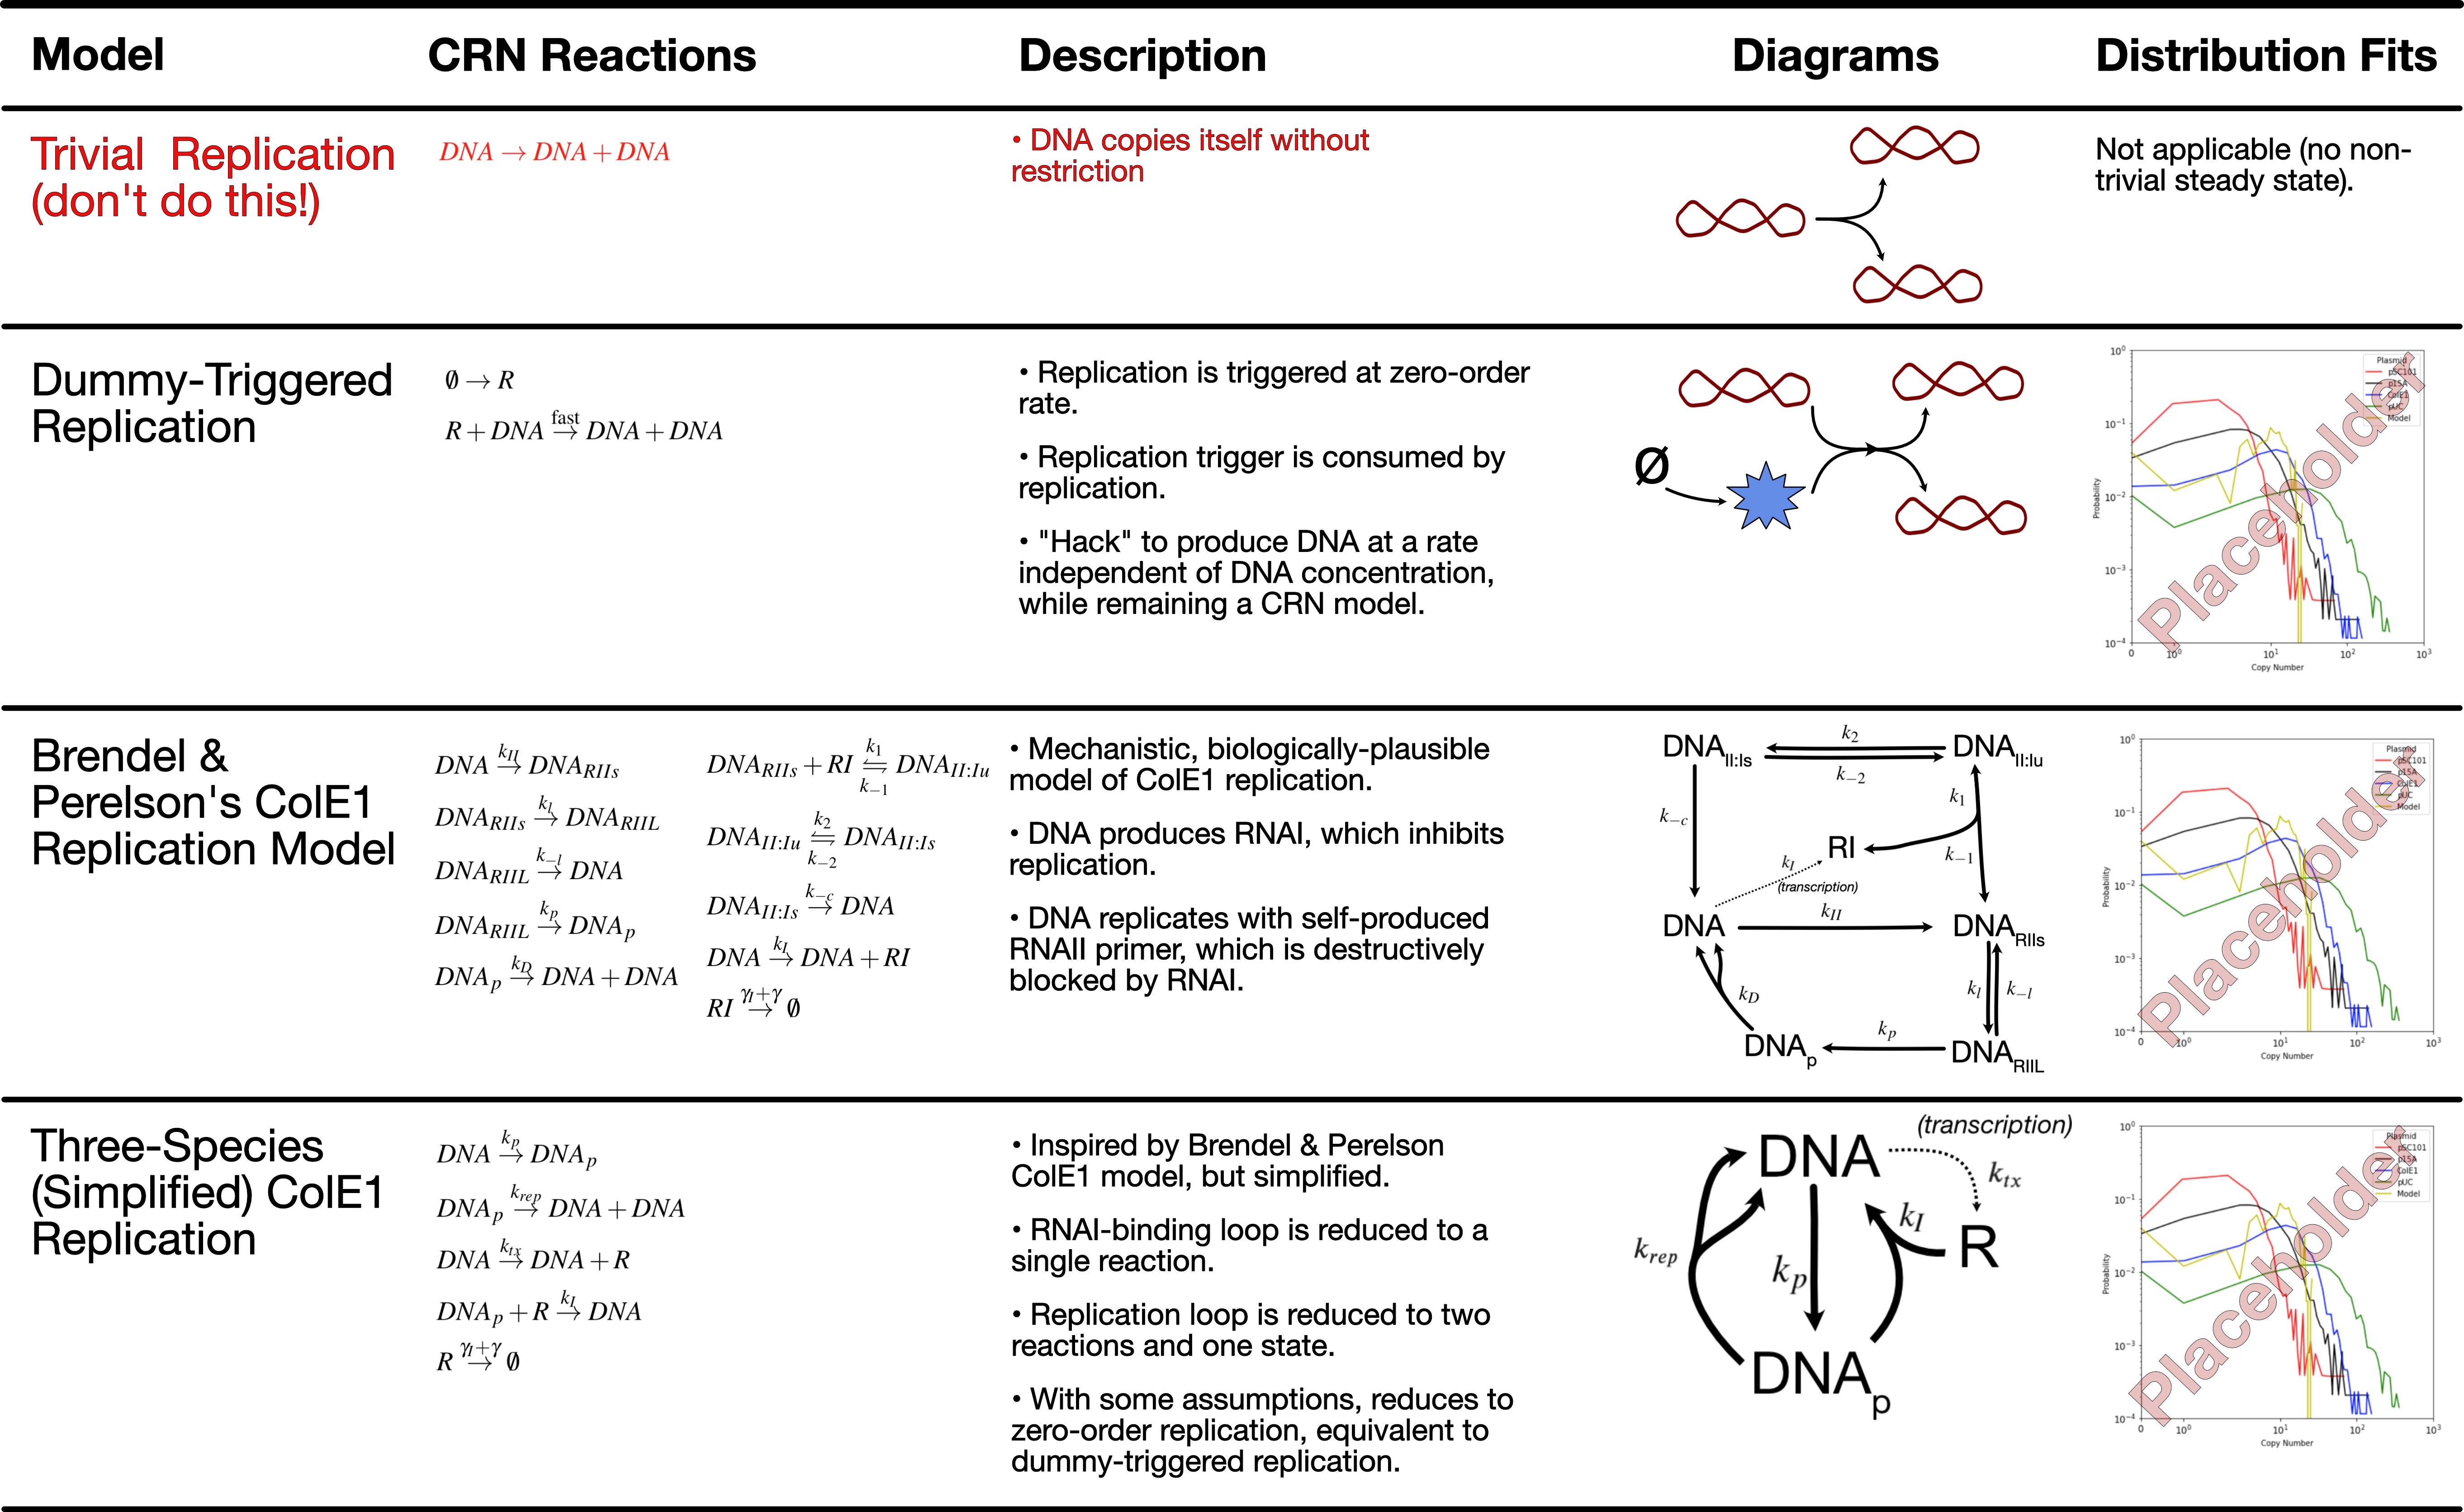
\includegraphics[width=8.5in, angle=90]{figures/main_table.png}
\label{fig:main_table}
\end{figure}
\pagebreak
%\eject

%\renewcommand\tabcolsep{6pt}
%\renewcommand\arraystretch{1}
%\begin{table}[H]
%\begin{tabular}{p{4cm} p{6cm} p{9cm} p{5cm} p{6.5cm} p{2cm}}
%\toprule
%\textbf{Model} 
%	& \textbf{CRN Reactions}
%	& \textbf{Description}  
%	& \textbf{Diagram} 
%	& \textbf{Steady State Distributions} 
%	& \textbf{Simulation Time} \\ \midrule
%\textcolor{red}{Trivial Replication (don't do this!)}
%	& \textcolor{red}{$DNA \to DNA + DNA$ }
%	& \begin{itemize}\color{red}\item DNA copies itself without restriction. \end{itemize}
%	&  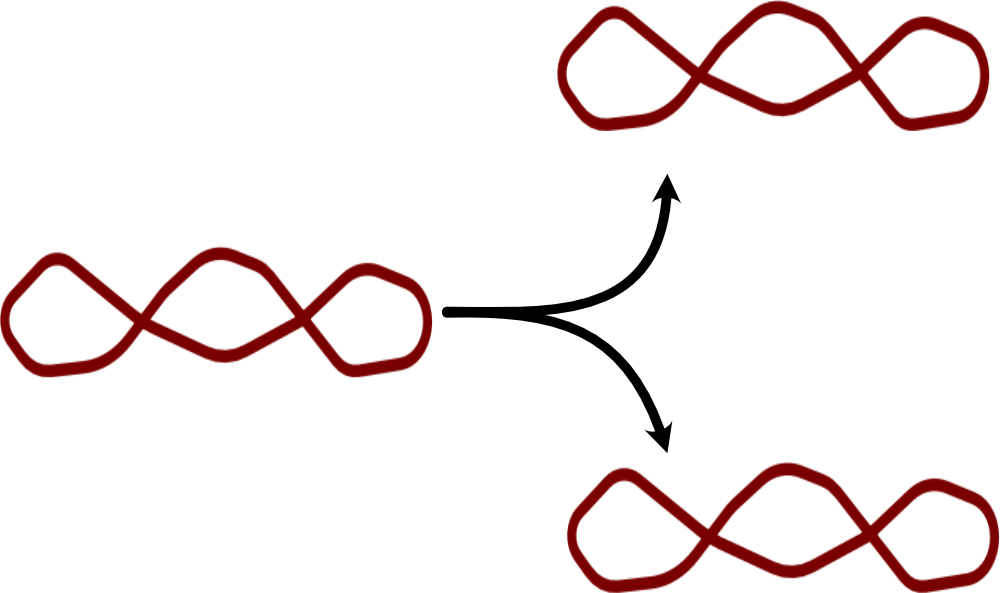
\includegraphics[align=c,scale=.5]{figures/intuitive_mockup.png}
%	&  \textcolor{red}{n/a}
%	&  \textcolor{red}{n/a} \\ \midrule
%Dummy Replication Trigger
%	& $\begin{aligned}
%		&\emptyset \to R\\
%		&R + DNA \overset{\text{fast}}{\to} DNA + DNA\\ 
%	      \end{aligned}$
%	& \begin{itemize} 
%		\item Replication trigger is produced at zero-order rate.
%		\item Replication trigger is consumed to replicate a DNA.
%		\item ``Hack'' to produce DNA at a rate independent of DNA concentration, while remaining a CRN %model.
%	   \end{itemize}
%	&     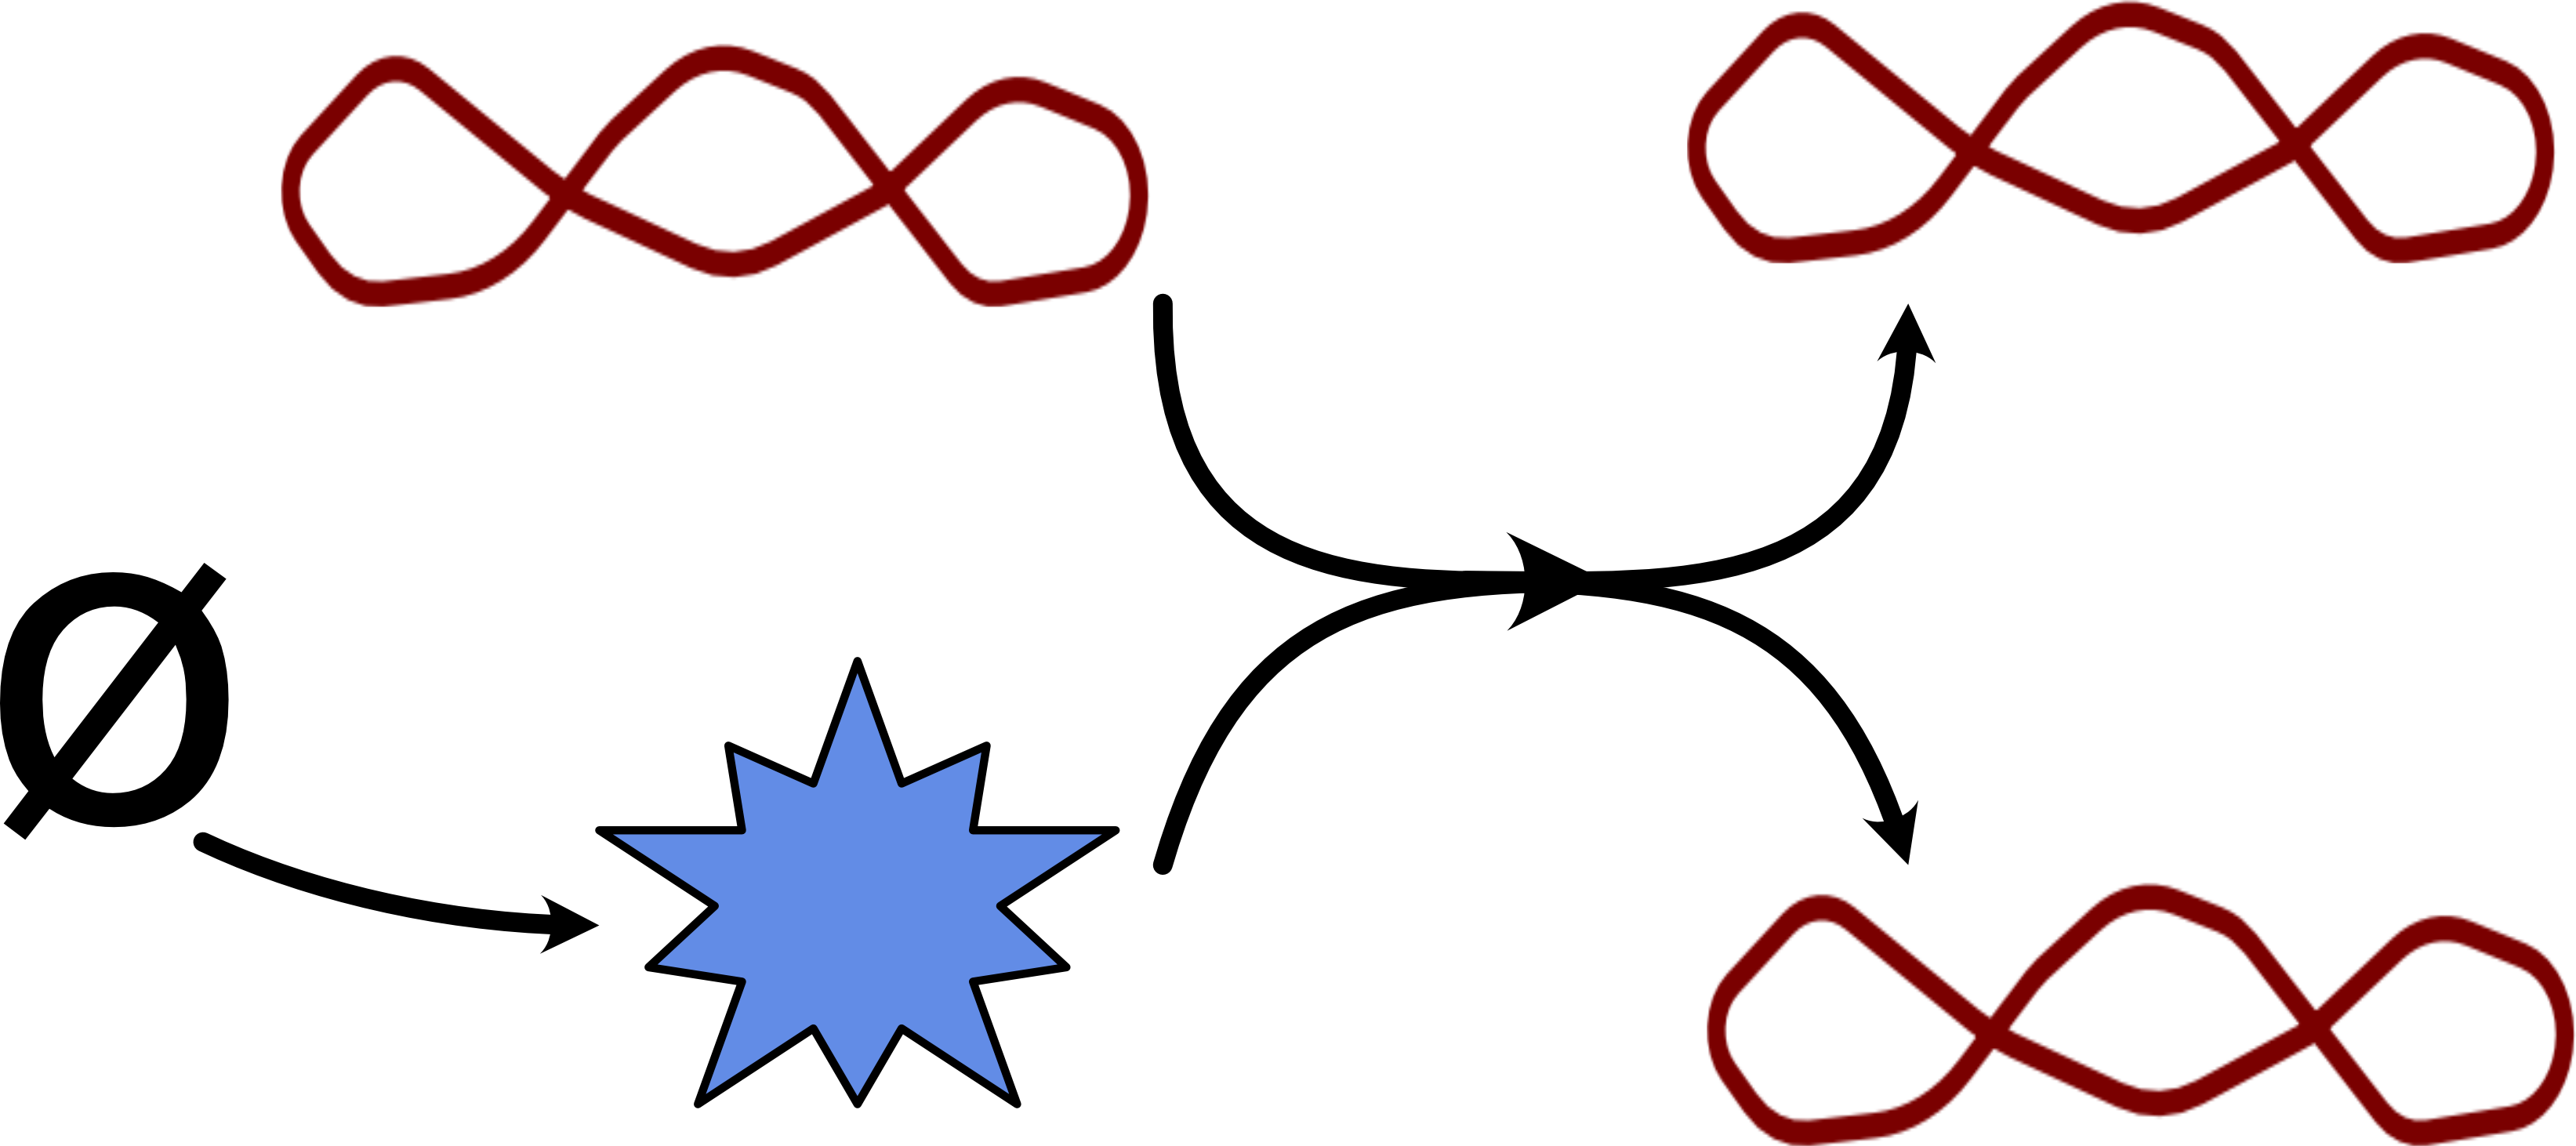
\includegraphics[align=c,scale=.15]{figures/dummy_mockup.png}                                               
%	&     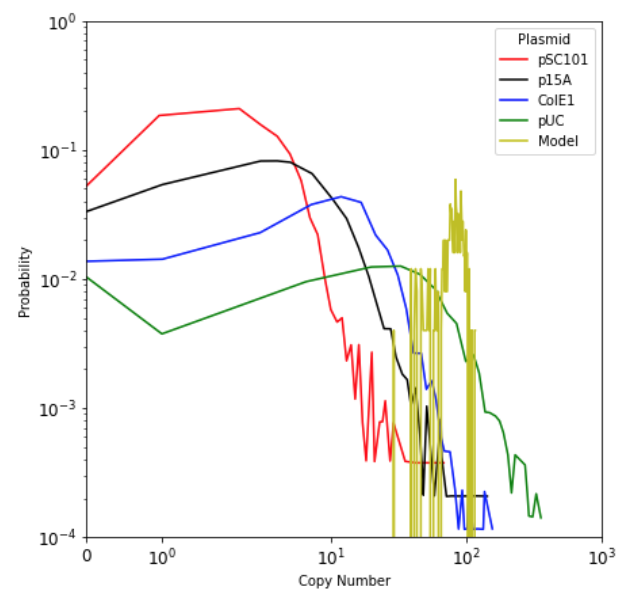
\includegraphics[align=c,scale=.5]{figures/distribution_mockup_0.png}                                 
%	&          1x                \\ \midrule
%Brendel \& Perelson ColE1 Model
%	&     {$\begin{aligned}[]
%		&DNA \overset{k_{tx}}{\to} DNA + RI\\
%    		&DNA \overset{k_{II}}{\to} DNA_{RIIs}\\
%    		&DNA_{RIIs} \overset{k_l}{\to} DNA_{RIIL}\\
%    		&DNA_{RIIL} \overset{k_{-l}}{\to} DNA\\
%    		&DNA_{RIIL} \overset{k_p}{\to} DNA_p\\
%    		&DNA_p \overset{k_D}{\to} DNA + DNA\\
%    		&DNA_{RIIs} + RI \underset{k_{-1}}{\overset{k_1}{\leftrightharpoons}} DNA_{II:Iu}\\
%    		&DNA_{II:Iu} \underset{k_{-2}}{\overset{k_2}{\leftrightharpoons}} DNA_{II:Is}\\
%    		&DNA_{II:Is} \overset{k_{-c}}{\to} DNA\\
%   		&DNA \overset{k_I}{\to} DNA + RI\\
%    		&RI \overset{\gamma_I + \gamma}{\to} \emptyset
%  		\end{aligned}$} 
%	&  \begin{itemize}
%		\item Mechanistic, biologically-plausible model of ColE1 plasmid replication.
%		\item DNA produces RNAI, which controls copy number.
%		\item DNA  replicates using a self-produced RNAII primer.
%		\item RNAII is destructively blocked by a RNAI. High RNAI $\to$ less replication.
%	    \end{itemize}
%	& 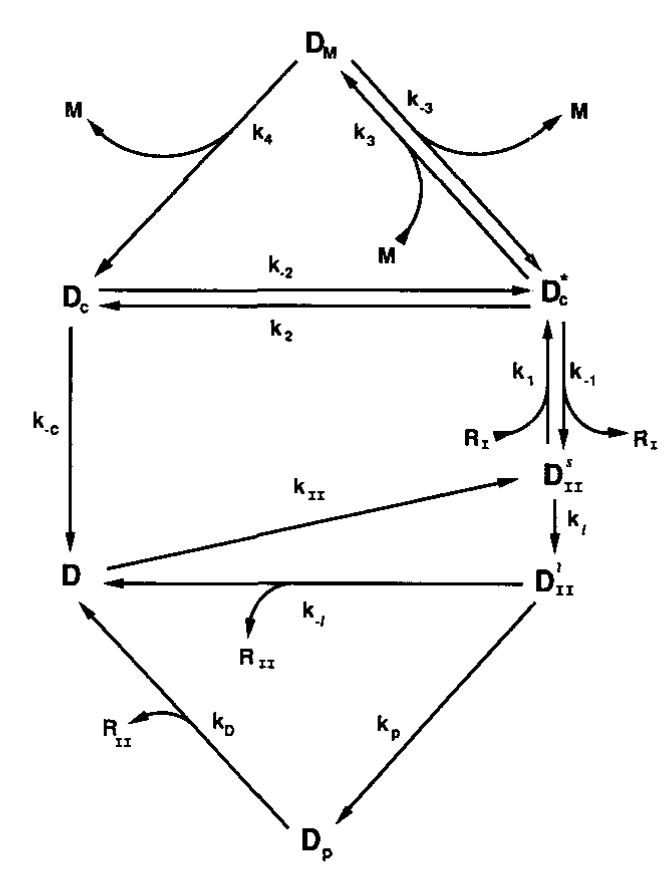
\includegraphics[align=c,scale=.5]{figures/BP_mockup.png}  
%	& 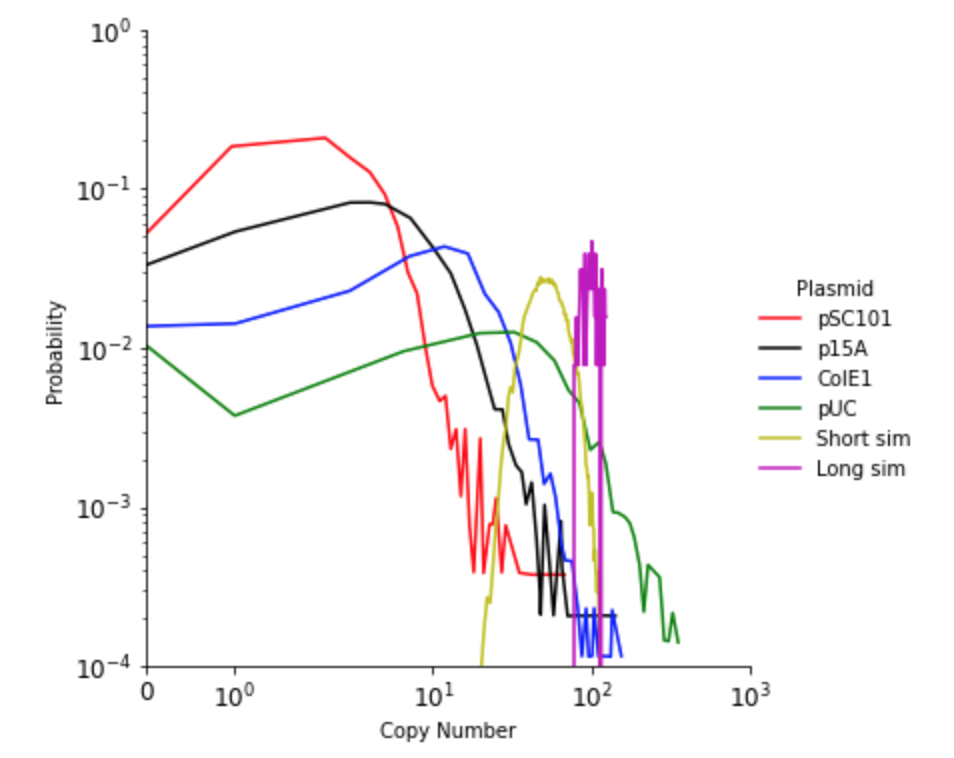
\includegraphics[align=c,scale=.4]{figures/distribution_mockup.png} 
%	& 55x  \\ \midrule
%Three-Species Reduced ColE1Model
%	&  {$\begin{aligned}[]
%    		&DNA \overset{k_p}{\to} DNA_p\\
%    		&DNA_p \overset{k_{rep}}{\to} DNA + DNA\\
%   		 &DNA \overset{k_{tx}}{\to} DNA + R\\
%   		 &DNA_p + R \overset{k_I}{\to} DNA\\
%   		 &R \overset{\gamma_I + \gamma}{\to} \emptyset
%		\end{aligned}$}      
%	& \begin{itemize}
%		\item Biologically-inspired model of ColE1 replication, but simplified.
%		\item RNAI-bound loop is reduced to one state.
%		\item Replicating DNA with elongated (un-blockable) RNAII reduced to one state.
%	   \end{itemize}
%	& 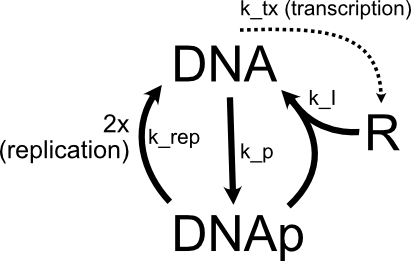
\includegraphics[align=c,scale=1.2]{figures/simpleBP_mockup.png}  
%	& 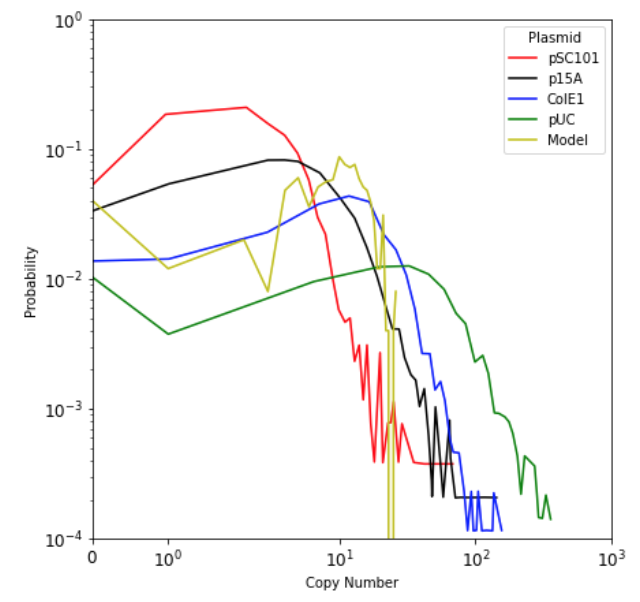
\includegraphics[align=c,scale=.5]{figures/distribution_mockup_2.png} 
%	&  48x \\ \bottomrule
%\end{tabular}
%\end{table}
%\pdfpagewidth=20in \pdfpageheight=18in
%\clearpage
%
%
%\eject \pdfpagewidth=8.5in \pdfpageheight=11in

% MODEL DETAILS
\section{Model Details}

\subsection{What is this?}

This document is a quick guide to several different effective ways to add a replicating DNA species to a Chemical Reaction Network (CRN) model of a biocircuit, along with a few warnings about how \emph{not} to do it. We've provided three different DNA replication models of varying complexity and biological plausibility.

\subsection{What's an ``effective'' model of DNA replication?}

This guide is written for engineers and biologists who need some way to represent replicating DNA in their biocircuit models. In most cases, the most important feature of such a model is that it can hold a DNA species at (roughly) a constant concentration. We will consider a model that can do this a ``good'' model. An even better property of a model of replicating DNA is to produce a realistic \emph{distribution} of copy numbers over time and across a simulated population -- we will also consider how well models can do this in \hyperref[S:evaluation]{Section \ref{S:evaluation}}.

For the purposes of this document, an ``effective'' or ``good'' model of replicating DNA is a CRN model that can stably hold a DNA species at a roughly-fixed copy number. A \emph{really} good model of replicating DNA is a CRN model that accurately reproduces the real-world steady-state copy number distribution of a DNA species. 

This document was written to help engineers who might need to model replicating DNA. As such, ``effective'' does \emph{not}, for the purposes of this document, imply that the model accurately represents a real mechanism of DNA replication, or that it can provide any insight into natural replication systems. 

\subsection{Who is this for?}

This guide is intended for synthetic biologists and systems biologists who use CRN models and who might need to model a biocircuit with explicitly-tracked DNA species. In particular, it is intended for those working with stochastic models -- for deterministic models, the trivial model is probably fine (see \hyperref[sss:deterministic_ignore]{Section \ref{sss:deterministic_ignore}}).

\subsection{Why should I care?}

	See \hyperref[S:motivation]{Section \ref{S:motivation}}.

\subsection{What's wrong with the trivial model? Why shouldn't I use it?}

The trivial replication model is the most obvious way to model replication of a DNA species $DNA$ -- simply have $DNA$ copy itself from time to time at some rate, say $\alpha$. This can work just fine in the deterministic limit of high concentrations and ample mixing -- together with a dilution term $DNA \overset{\gamma}{\to} \emptyset$, it translates to an ODE like 

$$\frac{DNA}{dt} = (\alpha - \gamma) DNA$$.

This has a steady-state value when $\alpha = \gamma$, though we might be suspicious that it is not a \emph{well-defined} steady state -- whatever concentration $DNA$ starts at, it will stay at. 

The problem is that in anything other than the infinite deterministic limit, the trivial replication mechanism doesn't keep copy number stable. Figure \ref{fig:model_trajectories}A shows what you get if you try simulating this mechanism in a stochastic regime, using Gillespie's Stochastic Simulation Algorithm (SSA) \cite{Gillespie1977}.

\begin{figure}[!ht]
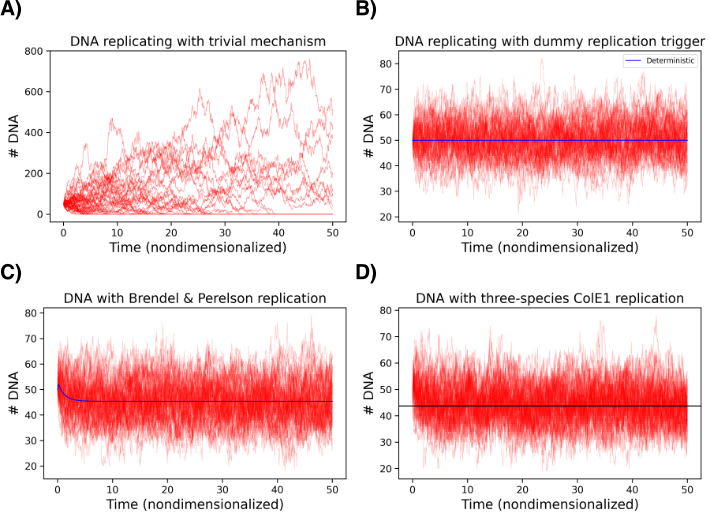
\includegraphics[width=5in]{figures/good_rep_trajectories.png}
\caption{Typical dynamics of DNA replicating with different mechanisms. Each line is one simulated cell. \textbf{A)} Trivial $DNA \to DNA + DNA$ mechanism. The distribution does not go to steady state unless all cells lose their plasmids -- cells with high DNA concentration will tend to gain copies indefinitely. \textbf{B)} Dummy-triggered replication. \textbf{C)} Brendel \& Perelson's ColE1 replication mechanism. \textbf{D)} Three-species reduced ColE1 replication mechanism.}
\label{fig:model_trajectories}
\end{figure}

Each line in Figure \ref{fig:model_trajectories}A is a sample trajectory for a DNA species starting at 50 copy number and allowed to run with $\gamma = \alpha = 1$. Cell growth is implemented with the dilution reaction (i.e., this is a BioSCRAPE SSA simulation, not a BioSCRAPE lineage simulation). Fifty independent results are shown -- most of them collapsed down to copy number 0 by about $t=150$. 

The trivial replication mechanism is not stable. Any fluctuation to a higher copy number leads to an increase in overall DNA replication rate, which leads to higher copy number. On the other hand, fluctuations to lower copy number reduce overall DNA replication rate, which leads to lower copy number. A DNA species replicating this way is effectively undergoing a random walk in concentration with an absorbing state at 0, which is why real self-replicating DNAs either replicate much faster than dilution (and so grow indefinitely until they use up one or another of their host's resources) or employ a copy number control system of some kind. 

\subsection{Real replication involves delays. Can't we salvage the trivial model by adding a delay on the order of cell replication time?}

Not really. Adding a delay doesn't solve the inherent instability of the trivial model. It just makes the DNA population disappear/explode in discrete bursts, instead of more-or-less continuously.

\subsection{What in the world is that species R in the first model? What kind of molecule is the trigger supposed to represent?}

$R$ is a hack to get zero-order $DNA$ production while keeping them model a CRN. It does not represent any real molecule.

The dummy replication trigger model represents an attempt to fix the fundamental problem of the trivial replication mechanism (\emph{i.e.}, that it fails because first-order self-replication coupled with first-order dilution is unstable). The trivial mechanism's ODE description looks like $\frac{dDNA}{dt} = (\alpha - \gamma) DNA$, which has no non-zero steady state. If replication were, instead, zero-order (that is, constant with DNA count rather than proportional to it), then we would have something more like $\frac{dDNA}{dt} = \alpha - \gamma DNA$, which has steady state $\alpha / \gamma$. 

The problem is that a CRN can't directly represent zero-order self-replication because the reaction $DNA \to DNA + DNA$ will always have a rate dependent on the concentration of DNA! A CRN can, however, \emph{emulate} zero-order replication by tying a normal replication reaction to the zero-order production of a rate-limiting dummy molecule that is consumed by the reaction.

We recommend this model for most applications for any DNA with large enough copy number that it won't readily be lost (this threshold is parameter-dependent, but as a guideline, if a DNA doesn't need active partitioning to maintain, this model is probably fine). It isn't \emph{just} a hack to get meaningful steady-state behavior -- in the right parameter regime, Brendel \& Perelson's model of ColE1 plasmid replication reduces to essentially this model (see section \ref{sec:simple_bp_reduction}).

\subsubsection{Why use the dummy trigger? Why not just have plasmid directly replicate at zero-order rate?}

I settled on the dummy trigger mechanism because it was trivial to implement in CRN-based simulators. If you are using a simulator where you can assign arbitrary (non-CRN-like) propensities to reactions, then you can certainly have the reaction $DNA \to DNA + DNA$ occur at zero-order propensity and omit the dummy trigger species. 

Even staying strictly within the world of CRNs, in many cases, you could instead use the simpler model $\emptyset \to DNA$. The dummy replication trigger model is more general, however, and can handle some cases where direct zero-order DNA production fails, such as:

\begin{itemize}
	\item If you need to do something other than simply make a new plasmid during replication (for example, when \hyperref[ss:CRISPRi]{replication triggers an unbinding event}), or 
	\item If you have more than one competing, inheritable DNA species (for example, when tracking a \hyperref[ss:temporal_gate]{circuit using replicating DNA modified by an integrase)}.
\end{itemize}

\subsubsection{The dummy trigger looks suspiciously like a DNA polymerase. Could you instead model replication using a limiting polymerase to keep replication zero-order?}

The simplest model of a DNA polymerase would look something like $DNA + \text{Polymerase} \to DNA + DNA + \text{Polymerase}$, which occurs at a rate proportional to the concentration of $DNA$. This is functionally identical to the trivial model, and is just as unstable.

You could instead use a Michaelis-Menten polymerase with reactions

$$DNA + \text{Polymerase} \leftrightarrow DNA:\text{Polymerase} \to DNA + DNA + \text{Polymerase}$$.

This polymerase model should approximate zero-order replication for (sufficiently) high-copy plasmids if the production reaction is sufficiently rate-limiting. This is arguably a more biologically \emph{plausible} model -- though notably, real-world plasmids typically use copy number control mechanisms beyond rate limitation by host polymerase, so it is not clear that this model's \emph{plausibility} should translate to better \emph{biological plausibility}.

\subsection{There's a lot going on in the Brendel \& Perelson model. What is this, and what are all those states?}

Real cells keep DNA concentrations constant. One principled way of modeling DNA replication is to simply describe how they do that. There are a number of different DNA copy control mechanisms, but one of the simplest and best-understood is the ColE1 copy number control system, described in model form by Brendel \& Perelson in 1993 \cite{Brendel1993}. 

Briefly, ColE1 plasmids replicate using a \emph{cis}-acting RNA primer, called RNAII. That primer can be blocked by a complementary RNA called RNAI, which is constitutively produced by the ColE1 plasmid. This means that the per-plasmid rate of ColE1 replication drops as the concentration of ColE1 plasmids increases, which gives ColE1 a finite steady state. 

In the absence of RNAI, a ColE1-based $DNA$ species are duplicated by initiation of RNAII transcription ($DNA \to DNA_{RIIs}$), elongation of RNAII ($DNA_{RIIs} \to DNA_{RIIL}$), attachment of a DNA polymerase to the RNAII-primed DNA complex ($DNA_{RIIL} \to DNA_P$), and, finally, replication by the attached DNA polymerase ($DNA_P \to DNA + DNA$). If a DNA polymerase does not bind to an elongated RNAII, the RNAII will be cleaved off, returning the plasmid to its initial state ($DNA_{RIIL} \to DNA$). 

ColE1 does, however, produce RNAI ($DNA \to DNA + RI$). RNAI can bind to RNAII while it's being transcribed, blocking elongation ($DNA_{RIIs} + RI \to DNA_{II:Iu}$). The RNAI:RNAII complex formed this way is unstable and can reverse easily, but can switch into a much more stable form ($DNA_{II:Iu} \to DNA_{II:Is}$) from which both RNAs can be cleaved off the plasmid by RNase action, resetting the plasmid ($DNA_{II:Is} \to DNA$). This serves as the negative feedback mechanism that lowers ColE1's replication rate as its copy number increases.

In their original description of this model, Brendel and Perelson also describe optional sequestration of the $DNA_{II:Is}$ state by \emph{Rom} binding, which leads to a lower steady state copy number \cite{Brendel1993}. Freudenau \emph{et al} further extend this model with additional feedback by uncharged tRNA, which occurs under starvation conditions, and experimentally parameterize the model. For simplicity, I omit these two extensions in this work.

\subsection{What's the relationship between the ``Brendel \& Perelson'' and the ``Reduced ColE1'' model?}

The reduced Brendel \& Perelson ColE1 model is my attempt to capture the most important phenomenological features of the Brendel \& Perelson model using fewer DNA states and fewer reactions (a little under half of each). In the three-species model, DNA still produces a regulatory RNA species $R$. It can initiate replication by going into a state $DNA_P$. From here, it can either finish replicate ($DNA_P \to DNA + DNA$) or be reset by consuming an RNAI molecule ($DNA_P + R \to DNA$). 

\subsection{What's the relationship between the ``Reduced ColE1'' model and the ``dummy replication trigger'' model?}\label{sec:simple_bp_reduction}

Under realistic parameter regimes (specifically, when $R$ dynamics are fast and $k_p$ is relatively fast compared to $k_{rep}$), this three-species ColE1 model can be approximated by a single-species model equivalent to the dummy-triggered replication model with replication rate $k_{rep}k_p(\gamma + \gamma_I) / (k_I(k_{tx} - k_p))$. 

This approximation requires:
\begin{enumerate}
	\item Dynamics of creation and destruction of $R$ must be fast (i.e., $R$ must be at quasi-steady state compared to $DNA$ and $DNA_p$. 
	\item Replication must be bottlenecked by the $DNA_p \to DNA + DNA$ reaction (i.e., $k_p \gg k_{rep}$). This is true for the three-species model with parameters fit against simulations from the full Brendel \& Perelson ColE1 model.
	\item $k_{tx} > k_p > \gamma$ and $k_{rep} > \gamma$ (required for stability of the three-species ColE1 model). 
\end{enumerate}

Since $R$ dynamics are fast, we'll assume that $R$ is at quasi-steady state:

$$\frac{dR}{dt} = k_{tx} DNA - (\gamma+\gamma_I)R - k_I DNA_p R$$

$$\text{At steady state: } R = \frac{k_{tx}DNA}{(\gamma+\gamma_I) + k_IDNA_p}$$

Because $k_{rep}$ is, by assumption, relatively slow, we can think also consider the quasi-steady state concentration of $DNA_p$. At quasi-steady state, the equilibrium condition between $DNA$ and $DNA_p$ means that 

$$k_I*DNA_p*\frac{k_{tx}DNA}{(\gamma+\gamma_I) + k_IDNA_p} = k_p*DNA$$

so

$$DNA_p = \frac{k_p(\gamma + \gamma_I)}{k_I(k_{tx} - k_p)}$$

Surprisingly, we have discovered that the concentration of $DNA_p$ is roughly \emph{constant} regardless of the copy number of the plasmid. As long as this is true, the rate of replication (i.e., the rate at which $DNA_p$ goes to $2DNA$) is 

$$k_p * DNA_p = \frac{k_{rep}k_p(\gamma + \gamma_I)}{k_I(k_{tx} - k_p)}$$.

Since this is constant, we're back to the zero-order (e.g., dummy-triggered) replication model where DNA species replicate at a constant, $DNA$-independent rate! This zero-order, one-species reduced model will bring DNA to the same copy number and usually has behavior qualitatively very similar to the three-species model (Fig. \ref{fig:model_reduction_examples}).

\begin{figure}[!ht]
\centering
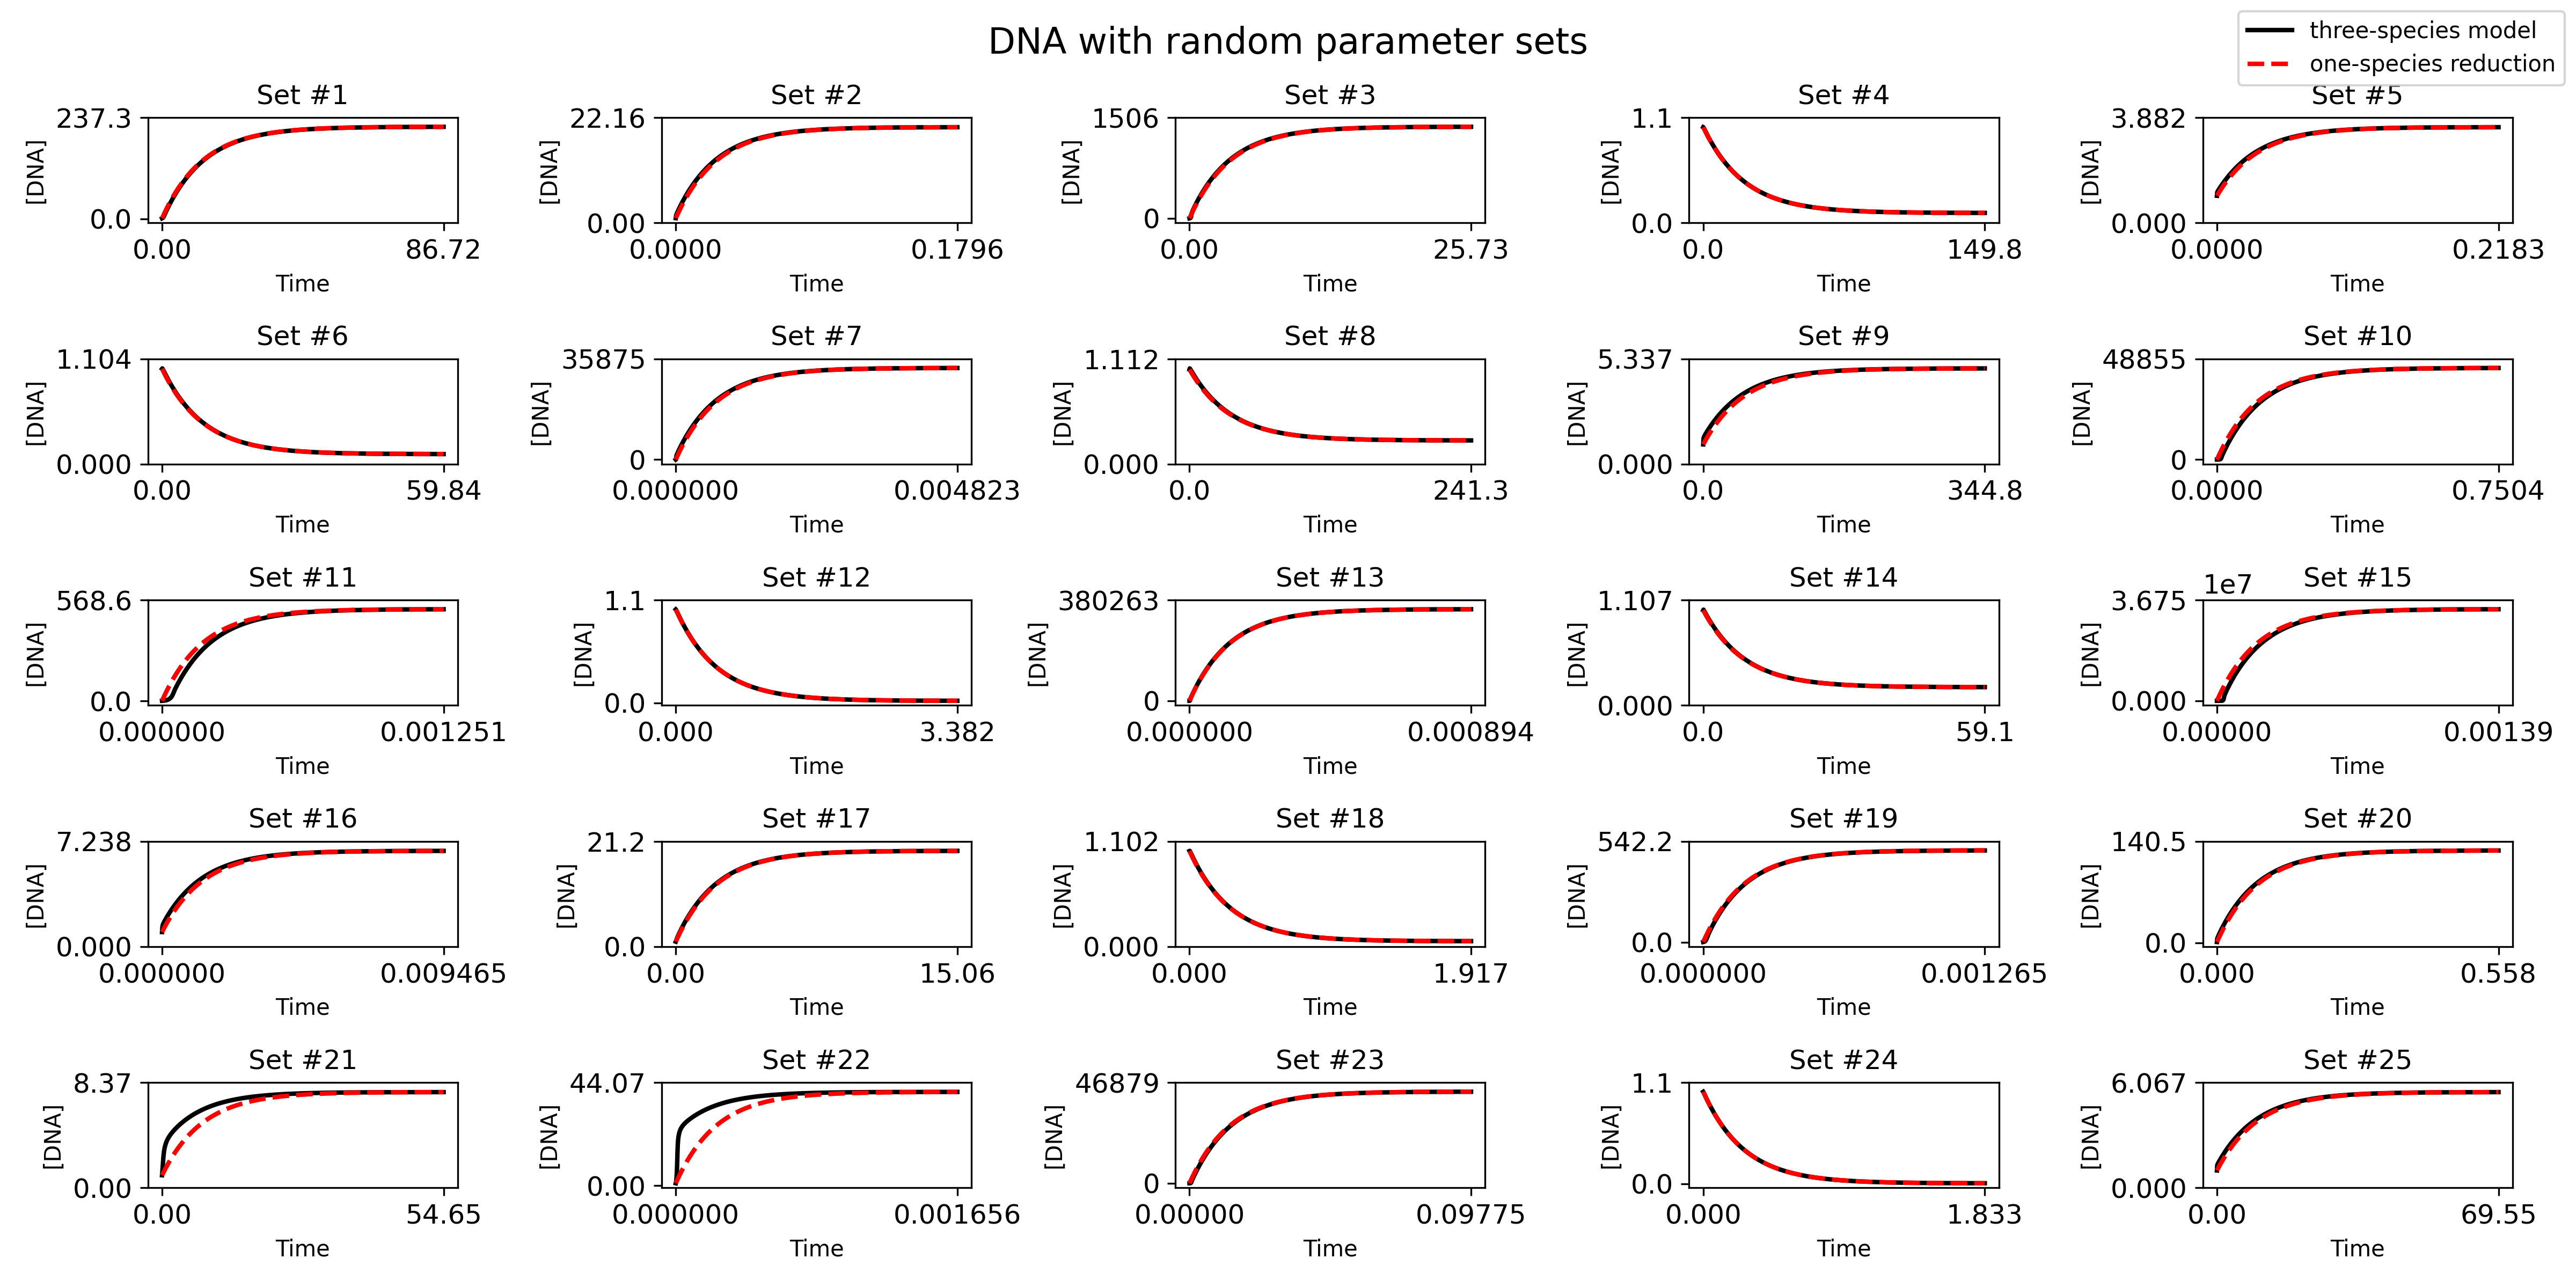
\includegraphics[scale=.35]{figures/model_reduction_examples.png}
\caption{Simulated trajectories of replicating DNA the three-species ColE1 model (black lines), with trajectories for the equivalent one-species reduced model (dashed red lines), for 25 random parameter sets chosen so that DNA has a finite, nonzero steady state and $k_p > k_{rep}$. }
\label{fig:model_reduction_examples}
\end{figure}

Note that in the opposite regime, where $k_{rep} \gg k_p$, a similar reduction can be made to a single-species model where DNA replicates at rate

$$\frac{k_p}{1 + \beta DNA}\text{, where } \beta = \frac{k_I k_{tx}}{k_{rep}(\gamma + \gamma_I)}$$

See the ipython notebook ``simple\_bp\_model\_reduction.ipynb'' in the code accompanying this document for more details.
% EVALUATING MODELS
\section{Evaluating Models}\label{S:evaluation}

\subsection{What's going on in the ``steady-state distributions'' plots?}

These plots demonstrate how closely the distribution of DNA copy numbers predicted by each model hews to real-world plasmid copy number data. Each color represents a different plasmid with a different copy number (and, in real cells, a different replication and copy number control mechanism). The dotted curves are empirical distributions measured by microscopy, while the solid curves are generated from BioSCRAPE lineage simulations run to a ``reasonable steady-state time.''

\subsection{What do the ``empirical distributions'' come from?} 

Empirical distributions were pulled from Figure 1e of \href{https://doi.org/10.1038/s41467-021-21734-y}{Shao \emph{et al}., Nature Communications 2021} \cite{Shao2021}. Copy numbers were measured by microscopy from approximately 1-2 thousand growing \emph{E. coli} cells bearing plasmids with binding sites for a GFP-fused transcription factor. I extracted frequencies from the figure using \href{https://automeris.io/WebPlotDigitizer/}{WebPlotDigitizer}, rounding each data point to the nearest whole plasmid copy number.

\subsection{How did you fit the models against the empirical distributions?}

\subsubsection{Dummy replication trigger}

The dummy replication trigger model only has one relevant parameter to tune, namely the production rate of $R$ (dilution rate is known and simply sets a timescale for the system, and the actual replication reaction merely needs to be fast enough to consume all $R$ quickly relative to other processes). For each empirical plasmid distribution, $R$ production rate was set to make the analytic steady state of the model ($R$ production rate divided by dilution rate) equal to the observed mean plasmid copy number. 

\subsubsection{Brendel \& Perelson, reduced Brendel \& Perelson}\label{sec:bp_howto_model}

The two Cole1 models required somewhat more complex fitting. In brief, parameters were optimized with Scipy on simulations using BioSCRAPE lineages in turbidostat mode.

For different parameter sets, I used BioSCRAPE lineages to grow a population out to a reasonable steady-state time with simulated copy number distributions extracted from the final time. Parameters were fit to each plasmid's empirical observations by computing least squared distance between the empirical distribution and simulated distribution at each copy number. 

Importantly, one of Shao \emph{et al}'s surprising findings was that large numbers of ``plasmid bearing'' cells do not appear to actually carry plasmids, \emph{even in the presence of antibiotic selection for those plasmids}. Therefore, for the ColE1 models to have any hope of closely reproducing real-world copy number measurements, my simulations must be able to handle common cases of total plasmid loss. As the models are written, with no other modification, plasmid loss is an absorbing state, and so all reasonable plasmid distributions would quickly tend toward total loss; therefore, I had to include some form of selection in my models.

BioSCRAPE allows the use of ``growth rules'' that tie growth (and replication) rate to the concentrations of molecules in the cell. We can therefore somewhat crudely represent antibiotic selection by applying the growth rule that cells stop growing when they have zero DNA. This allows cells with plasmid loss to persist in the population while also being subject to antibiotic selection, as by a bacteriostatic antibiotic (Shao \emph{et al} measure copy numbers of plasmids bearing ampicillin resistance). 

\subsection{Why don't you have steady-state distributions for the trivial model?}

The trivial model is unstable and has no steady state distribution, aside from the absorbing state of total plasmid loss. 

\subsection{So these models will hold plasmids at constant copy number ($\pm$ noise)?}

Almost. What ``copy number control'' mechanisms really act on is DNA \emph{concentration}, not copy number. For most purposes, this isn't a meaningful difference, but do note that the empirical distributions used in this report are distributions of \emph{copy number}, and the models were parameterized accordingly.

\subsection{How fast are these models to simulate, relative to each other?}

Table \ref{tab:speed} shows representative wall-clock run times for various stochastic simulations using each of the three replication models. As you can see, dummy-triggered replication is typically much faster than either ColE1 model, and different simulation conditions can make either ColE1 model faster than the other. 

All simulations were performed inside Jupyter Lab notebooks on a mid-2014 macbook pro (2.8 GHz Intel Core i5 processor, ample 1600 MHz DDR3 RAM). 

\begin{table}[hbt!]
\centering
\begin{tabular}{lllll}
\hline
System & \# Cells &  Dummy-Triggered & Full ColE1 & 3-Species ColE1\\
\hline
DNA only (non-lineage) &  50  & 0.27 sec & 13 sec & 10 sec\\
DNA only (guessed) & 64 & 0.35 sec & 11 sec & 7.5 sec \\
DNA only (hand-tuned) & 256 & 0.43 sec & 12 sec & 5.7 sec \\
DNA only (optimized) & 64 & .46 sec & 10 sec & 5.9 sec \\
5-node CRISPRlator & 1 & \#\#\# & \#\#\# & \#\#\# \\
5-node CRISPRlator & 64 & \#\#\# & N/A & N/A\\
TLG, copy number 30 & 1,056 & 5 hr, 14 min & N/A & N/A\\
TLG, copy number 100 & 1,056 & 17 hours, 9 min & N/A & N/A\\
\hline
\end{tabular}
\caption{Wall-clock run times for different simulations with each mechanism, where tested. TLG = Temporal Logic Gate. ``guessed'', ``hand-tuned'', and ``optimized'' refer to the parameter sets used for simulation. See Section \ref{ss:CRISPRi} for details of the 5-node CRISPRlator; see Section \ref{ss:temporal_gate} for details of the temporal logic gate (TLG).}
\label{tab:speed}
\index{tables}
\end{table}

\subsection{Which model should I use? Why?}

That depends on what you need from your model. If you just want to see the expected behavior of your circuit under stochastic assumptions with minimal fuss, I recommend using the dummy-triggered replication -- it is the simplest to implement of the working models, and runs much more quickly than either ColE1-based model. In the right parameter regimes, the dummy-triggered replication model approximates the other two quite well (see Section \ref{sec:simple_bp_reduction}). 

You might need to use a more realistic replication model if you anticipate coupling your circuit's DNA to other reactions (e.g., RNA degradation machinery) or if you anticipate a reviewer who asks you to use a more realistic replication model. In this case, either the Brendel \& Perelson ColE1 replication model or the reduced, three-species ColE1 replication model should suffice. You may want to try both to see which runs most efficiently; counterintuitively, sometimes the full ColE1 model is faster to run than the reduced model, although it is virtually always more effort to implement. 

\subsection{What's missing from these models?}

All of the models presented here assume random (binomial) partitioning of DNA. This is realistic for some DNA and not for others, and your milage may vary accordingly. Non-random partitioning can be added straightforwardly to Bioscrape lineages simulations, if desired. 

As written, these models also do not have any kind of antibiotic selection or other maintenance system, and nothing will stop a simulated DNA from dying out. This may be a problem for simulations of low copy number, especially since empirical measurements of plasmid copy number suggest that 0 is a perfectly reasonable number of plasmids to expect to find in a cell! The lineage simulations used for parameter-fitting include an added selection mechanism roughly mimicking ampicillin resistance (cells with no plasmid do not grow, and are likely to be pushed out by growing cells).

% MOTIVATION
\section{Motivation}\label{S:motivation}

\subsection{Why did you write this?}

I wrote this guide because I kept making models involving explicit DNA species, for a variety of reasons, and the simplest hacks I kept coming up with to handle them kept not working. This was doubly true when I started running stochastic simulations of biocircuits. I kept running into problems like transcription factors ``hiding'' from dilution by binding to DNA, or total plasmid loss, or plasmids spiraling out to infinite concentration and crashing Python. The standard modeling tools in my toolbelt didn't cover cases with replicating DNA.

Eventually I figured out a couple of replication mechanisms that didn't totally crash and burn or compromise on possibly-important kinetic details. Hopefully this document will save other modelers in similar situations the trouble.

\subsection{I've never had to model DNA replication in my models. Why would I ever need to?}

Most biocircuit models don't even include species representing DNA, much less model their replication. We can generally get away with this because of one or both of two common assumptions:

\begin{enumerate}
	\item \textbf{The concentration of DNA species is held constant by the cell.} Most DNAs (either chromosomal or plasmid) are copy-number controlled by more or less complex cellular processes, and we can usually assume that these processes are functioning properly in the background.
	\item \textbf{We do not need to track binding of species to the DNA.} Typically we assume that the actions of DNA-binding proteins (e.g. transcription factors) can be well-approximated by a Hill function or some other simple transfer function. The Hill assumption eliminates the need to explicitly track bound and unbound DNA states.
\end{enumerate}

As I've said, these assumptions are often good enough to use. However, there are some biocircuits that violate these assumptions. For example:

\begin{enumerate}
	\item When binding and unbinding of a transcription factor is slow relative to other processes (as can be the case with, for example, dCas9-based CRISPRi transcription factors \cite{Jones2017}), we may need to explicitly model binding and unbinding kinetics to understand whether or not that transcription factor will function in a circuit of interest. 
	\item Any time the state of a piece of DNA is malleable, inheritable, and important for circuit function, we may wish to track that DNA explicitly. Recombinase-based circuits that function by flipping, removing, or integrating chunks of DNA are a clear example of this case, particularly those such circuits on plasmids \cite{roquet2016, hsiao2016}.
	\item Any time we expressly wish to know the effect of the noise in copy number of a DNA species, we will likely want a way to track it. 
\end{enumerate}

Another case in which explicit DNA tracking might be useful would be if we wished to predict the transfer function of a transcription factor from purely kinetic parameterization, rather than empirically, though this is rare. Usually it is easier to put a transcription factor in a cell, induce its expression, and watch its effects than it is to directly measure its binding and unbinding rates; however, sometimes kinetic data may be available in the literature for a transcription factor for which there is no good direct transfer curve measurement, and modeling the transcription factor kinetically (rather than with a Hill assumption) may be appropriate.

\subsection{So these models are only useful for stochastic simulations?}\label{sss:deterministic_ignore}

More or less. In general, you can get away with using the trivial replication mechanism $DNA \to DNA + DNA$ if you're only using deterministic models, because you can exactly balance DNA replication against dilution. 

\subsection{When would you \emph{actually need} to model DNA replication? Give me a concrete example.}\label{ss:CRISPRi}

Here's one: the CRISPRlator (Figure \ref{fig:crispr_overview}).
	
\begin{figure}[!ht]
\centering
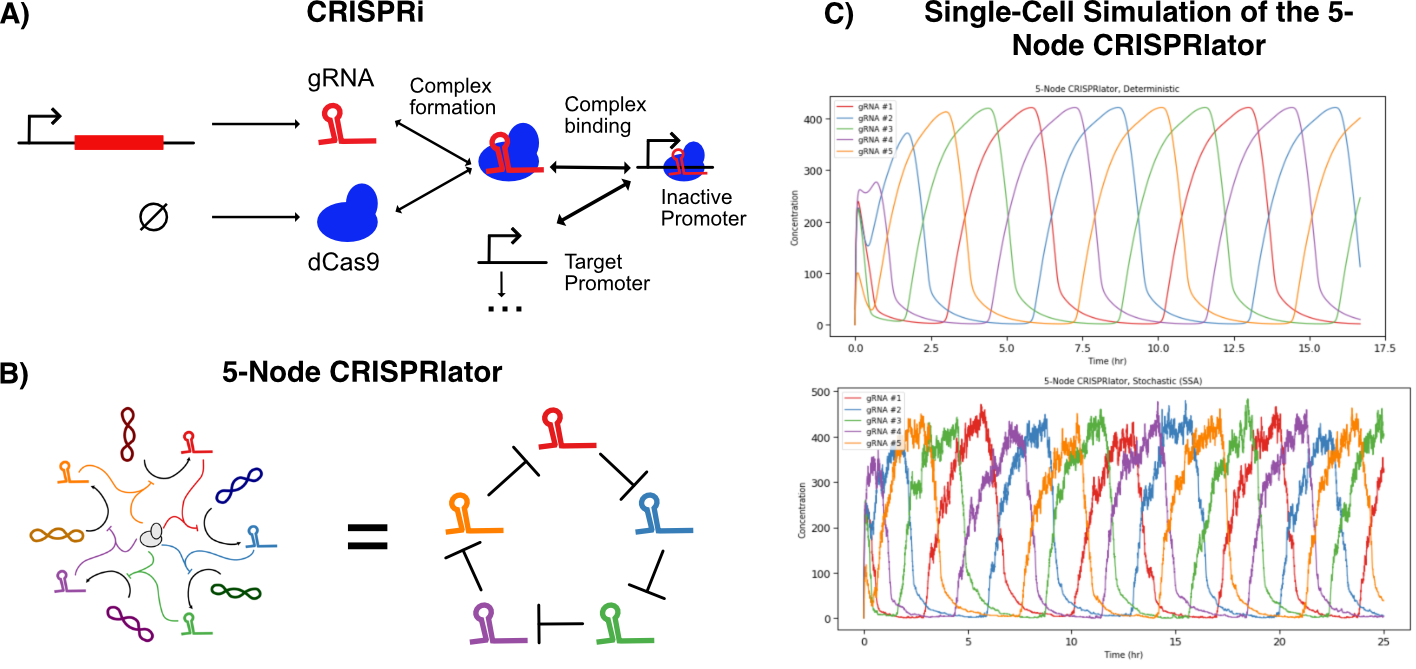
\includegraphics[scale=1]{figures/crispr_overview.png}
\caption{\textbf{A)} A simple model of general CRISPRi systems. Guide RNAs (gRNAs) complex with a shared pool of dCas9. dCas9:gRNA complexes bind to DNA targets, blocking transcription from those targets. Targets can be other gRNAs, as in the 5-node CRISPRi oscillator (CRISPRlator) \textbf{(B)}. \textbf{C)} Deterministic and stochastic (SSA, non-lineage) simulation of the 5-node CRISPRlator.}
\label{fig:crispr_overview}
\end{figure}

The CRISPRlator is just one example of a CRISPR interference (CRISPRi) circuit. CRISPRi circuits are transcriptional networks that use guide RNAs (gRNAs) that bind to catalytically deactivated dCas9 (dCas9) to form (theoretically) independent, orthogonal repressors \cite{Kiani2014, Nielsen2014, Gander2017}. The CRISPRlator in particular is a ring oscillator made of an odd number of gRNAs that repress each other in a cycle. With the right parameters, the CRISPRlator will naturally oscillate, with gRNAs activating in pulses, in turn \cite{Javier2020}.

CRISPRi is an appealing system for several reasons, but CRISPRi also has potential drawbacks compared to traditional gene expression networks \cite{Clamons2017, Zhang2018}. In particular, dCas9 has shockingly slow binding kinetics -- a single dCas9 molecule has been calculated to take an average of \emph{six hours} to find a single DNA target in an \textit{E. coli} cell, necessitating large numbers of targets and/or dCas9 molecules for circuits to operate on reasonable timescales \cite{Jones2017}. One might use simulation determine whether a particular CRISPRi circuit will function with particularly slow binding times. 

Note that to answer this question, we have to dispose of the usual Hill function approximation of gene repression -- one of the most common simplifying assumptions in the gene circuit literature -- because that assumption \emph{assumes} fast binding kinetics. To see the effects of slow binding kinetics, we have to explicitly model slow binding kinetics, which means explicitly tracking of bound and unbound DNA species. DNA replication might be a nice feature in such a model.

You may also simply want to know how fluctuations in plasmid copy number affect the performance of the CRISPRlator. Can the CRISPRlator function if DNA copy numbers fluctuate in ways consistent with noisy DNA replication? Can it survive random partitioning? Simulations with DNA replication could help answer those questions. 

\subsubsection{Is there \emph{really} no other way to model this circuit?}

For a deterministic or SSA simulation, you could assume that DNA concentrations are held constant by the cell (although you'll have to take care to account for the unbinding reactions implicit in balanced replication/dilution so that binding to DNA isn't a dilution-free `tax haven' for repressors!). This lets you model the CRISPRlator without any need for explicit DNA replication.

Things get tricker if you want to \emph{also} track the CRISPRlator in a lineage of growing, dividing cells. You may want to do this to, for example, see whether or not a CRISPRlator will stay synchronized across a population, or if you want to couple the CRISPRlator to another circuit in an \href{https://depts.washington.edu/soslab/gro/index.html}{agent-based model with spatial dynamics}. 

If you try to simulate the CRISPRlator in a lineage model without replicating DNA, you quickly run into a few problems. The first is that if a cell keeps a constant \emph{copy number} of a plasmid while \emph{growing in volume}, then the concentration of plasmid will consistently and unrealistically drop by a factor of two with every growth cycle. You will also run into a thorny question of how to add more plasmids to cells when they divide. The obvious thing to do is to instantaneously replicate all of the plasmids at cell division time, but this will create a bunch of un-repressed plasmids all at once, which can scramble the state of the CRISPRlator and kill oscillations. 

There may other ways to make a lineage model of the CRISPRlator work, but the best way I have found is to add explicit DNA replication mechanisms. 

\subsubsection{Does the CRISPRlator work in stochastic simulations with replicating DNA?}

Yes. Figure \ref{fig:crispr_results} shows representative simulations of a single-cell 5-node CRISPRlator using each DNA replication method. 

\begin{figure}[!ht]
\centering
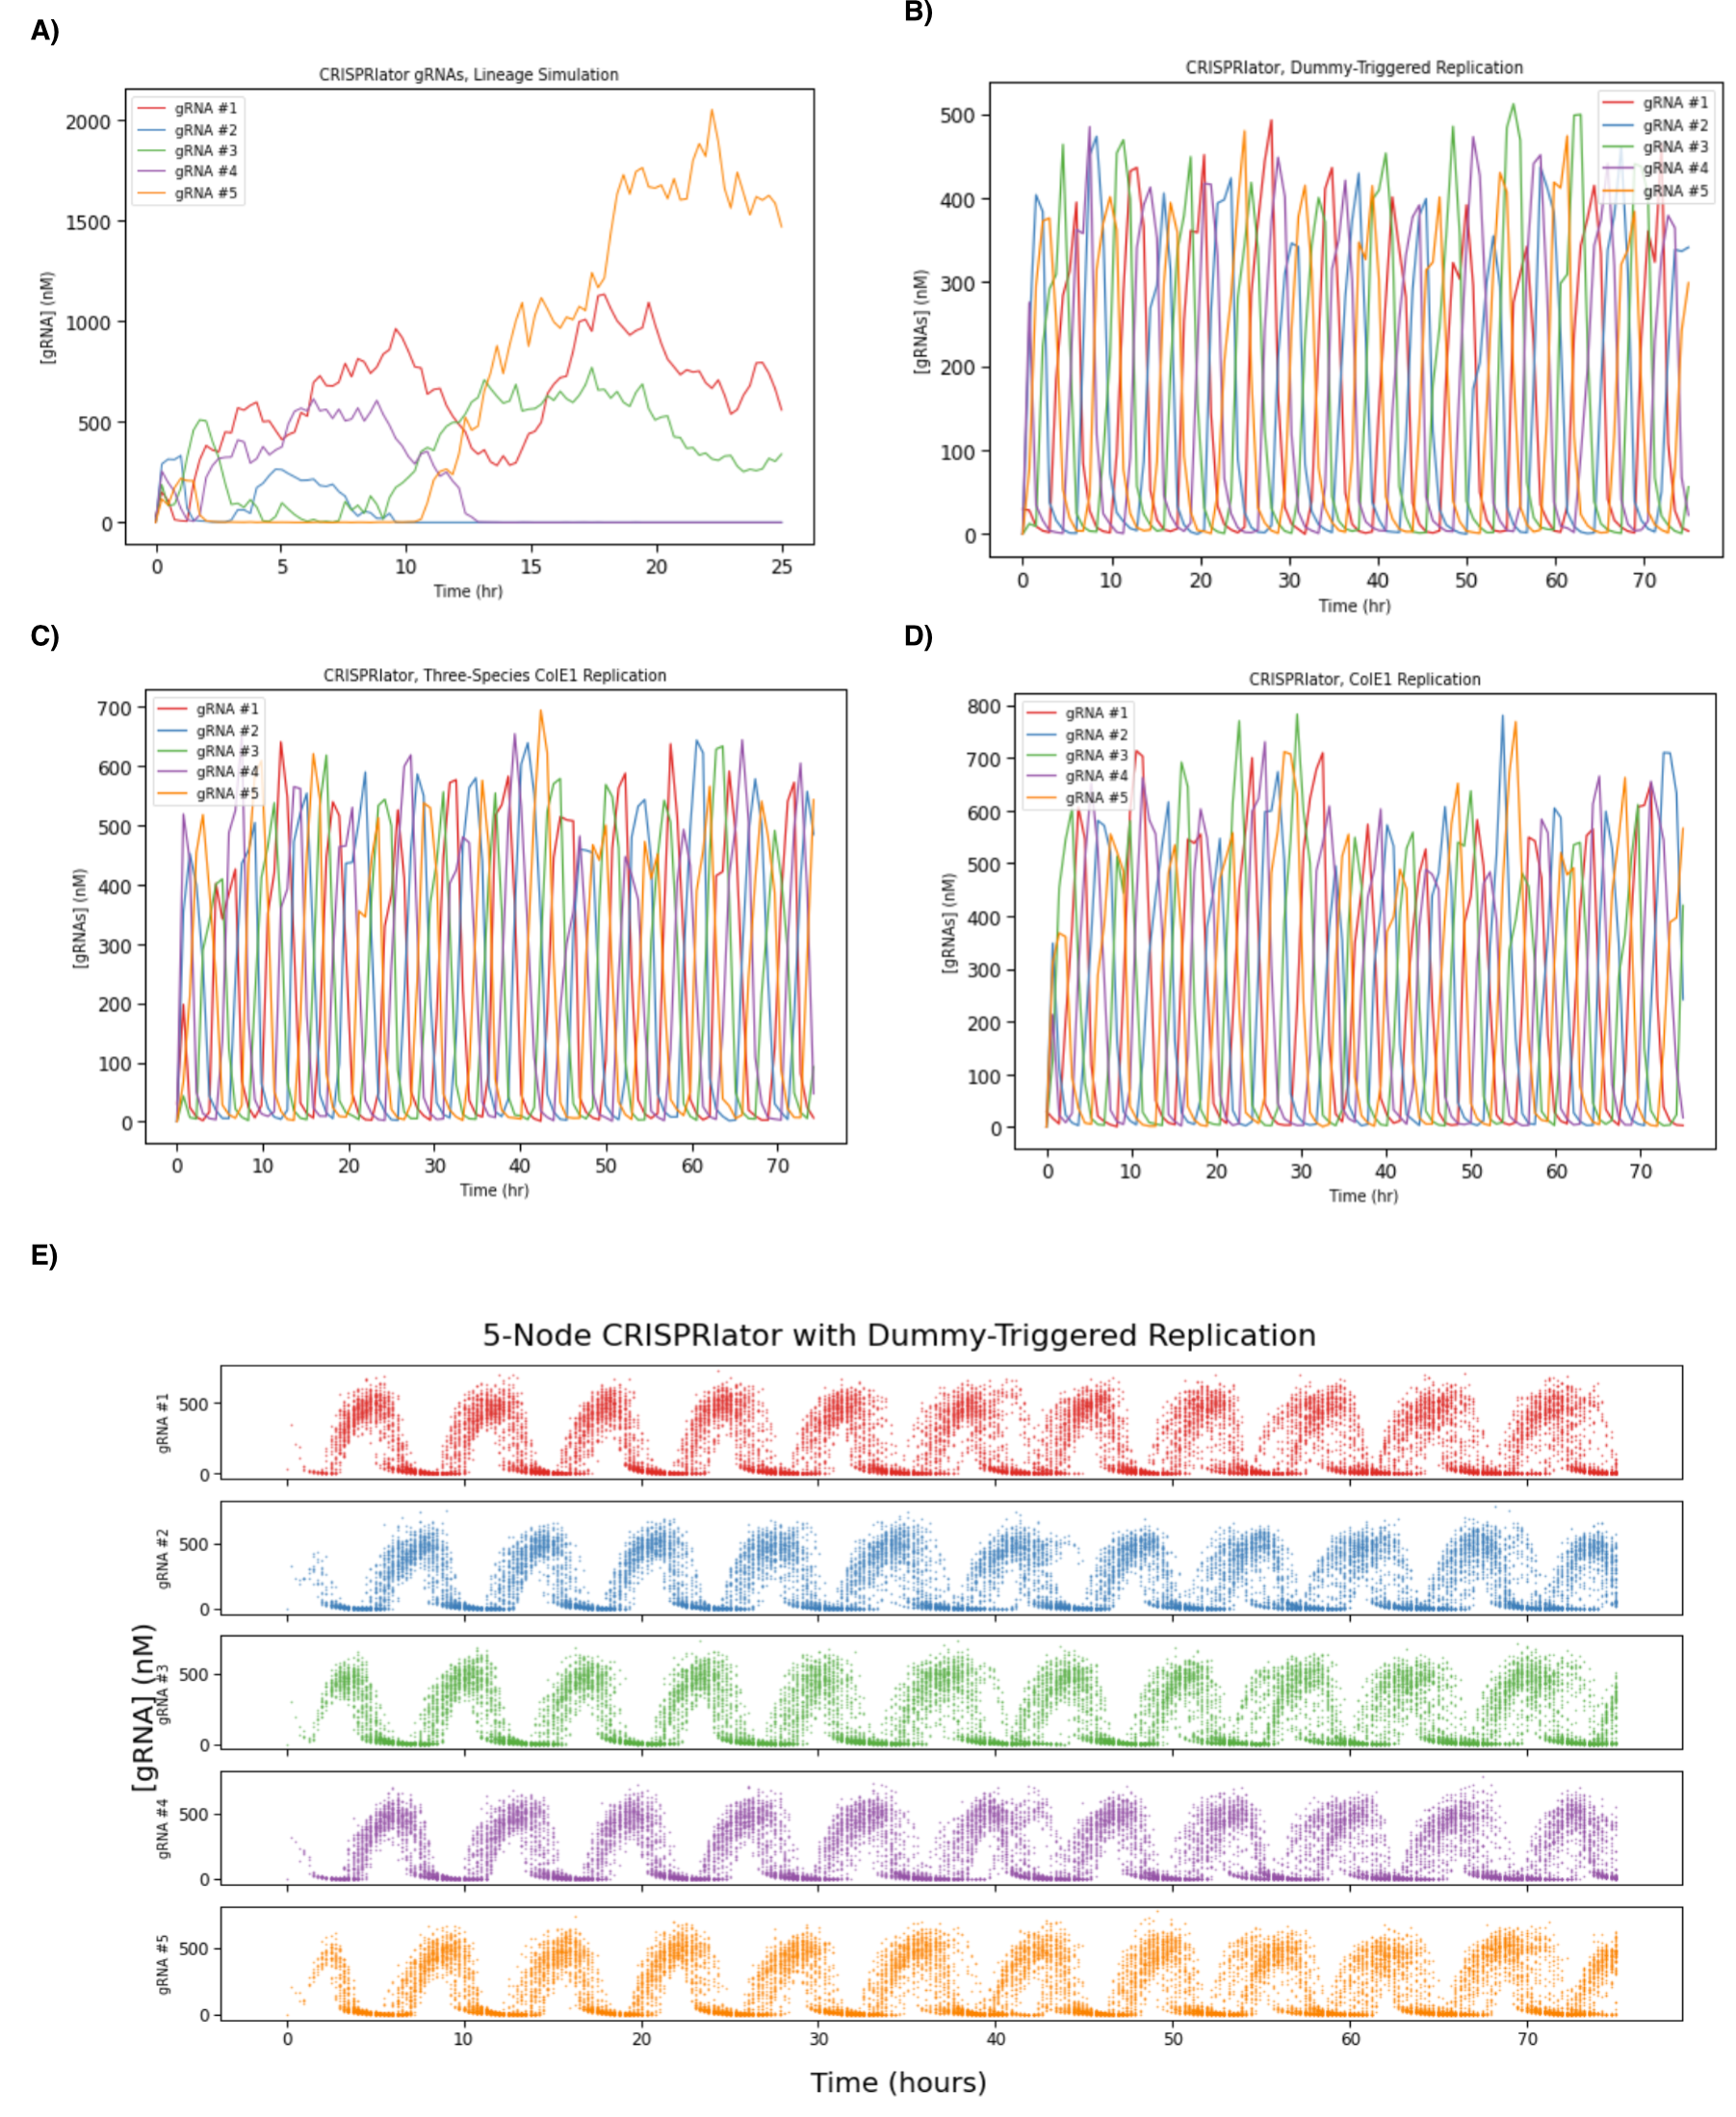
\includegraphics[scale=1]{figures/crispr_results.png}
\caption{The five-node CRISPRlator in a single growing cell with DNA replication modeled using \textbf{A)} the trivial replication model (note the shorter time scale), \textbf{B)} dummy-triggered replication, \textbf{C)} Brendel \& Perelson's ColE1 replication model, and textbf{D)} the simplified 3-species ColE1 replication model. Each line is a sum of the \emph{concentrations} of all species containing one of the five gRNAs. \textbf{E)} Lineage simulation of the 5-node CRISPRlator in growing, dividing cells over approximately 150 generations, with a population cap of 64 cells.}
\label{fig:crispr_results}
\end{figure}

More interestingly, we can now simulate lengthy lineages of growing, replicating cells expressing the CRISPRlator. Figure \ref{fig:crispr_results}E shows results from a lineage simulation using the dummy-triggered replication model parameterized identically to the one used for Figure \ref{fig:crispr_results}B. This simulation begins with a single cell, which grows and divides every doubling of cell size. The total population is capped at 64 by killing a random cell whenever a cell division would bring the population above 64. Each dot is the concentration of total gRNA for one of the five gRNA in one cell at one time. These simulations show that over 150 generations, the CRISPRlator remains largely coherent -- although increasingly less so as the simulation progresses (note the spread in the ``tails'' where each gRNA species falls to zero concentration). 

Finally, we can simulate the effect of dropping down the copy number of the plasmids bearing the CRISPRlator. Figure \ref{fig:crispr_results_2} shows representative traces from one of the five gRNAs in CRISPRlator variants on plasmids varying from single-copy to copy number ten. Guide RNA production rates are scaled so that the expected gRNA production rate are the same as in the simulations used for Figure \ref{fig:crispr_results}, and selection has been added to the models to counteract plasmid loss (see Section \ref{sec:bp_howto_model} for details). 

\begin{figure}[!ht]
\centering
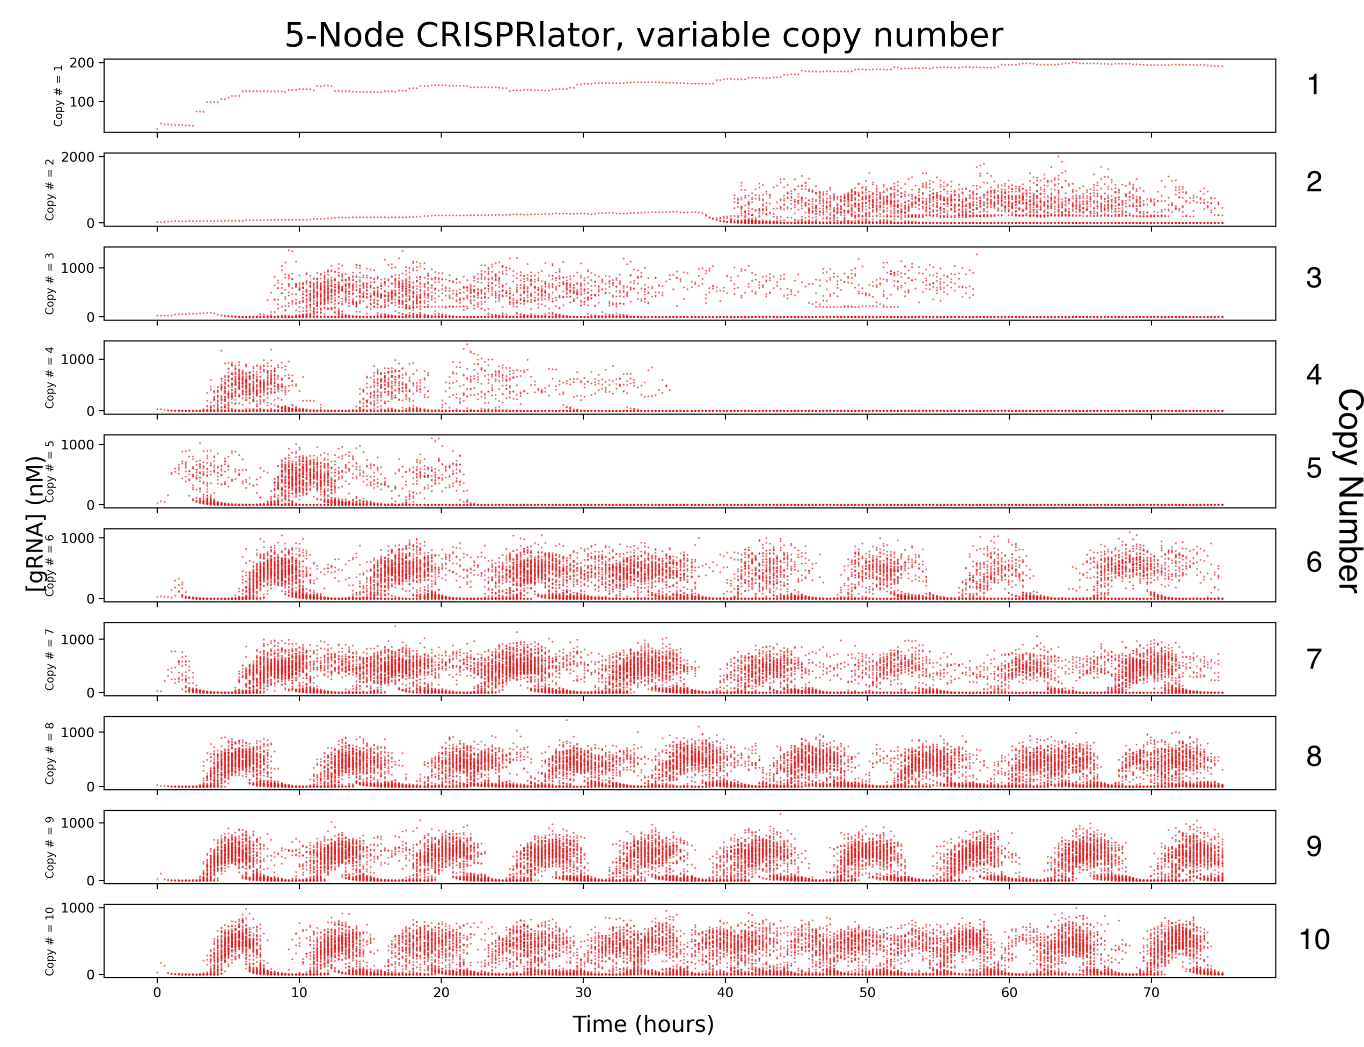
\includegraphics[scale=1]{figures/crispr_results_2.png}
\caption{5-node CRISPRlator at different copy numbers.}
\label{fig:crispr_results_2}
\end{figure}

\subsection{Okay, but that's just one example, and I don't care particularly about CRISPRi circuits. Can you give another concrete example?}\label{ss:temporal_gate}

Consider the integrase-based temporal logic circuit \citep{hsiao2016}, which is a special case of the general recombinase-based state machine \citep{roquet2016}. This circuit uses two different serine DNA integrases $intA$ and $intB$ under inducible control of molecules $A$ and $B$, respectively, to flip pieces of a shared reporter module. Induction of either integrase permanently alters the reporter module so that the circuit produces different outputs depending on whether it has been exposed to $A$ only, $B$ only, $A$ followed by $B$ ($A\Rightarrow B$), $B$ followed by $A$ ($B \Rightarrow A$), or no inducer at all.

\begin{figure}[!ht]
\centering
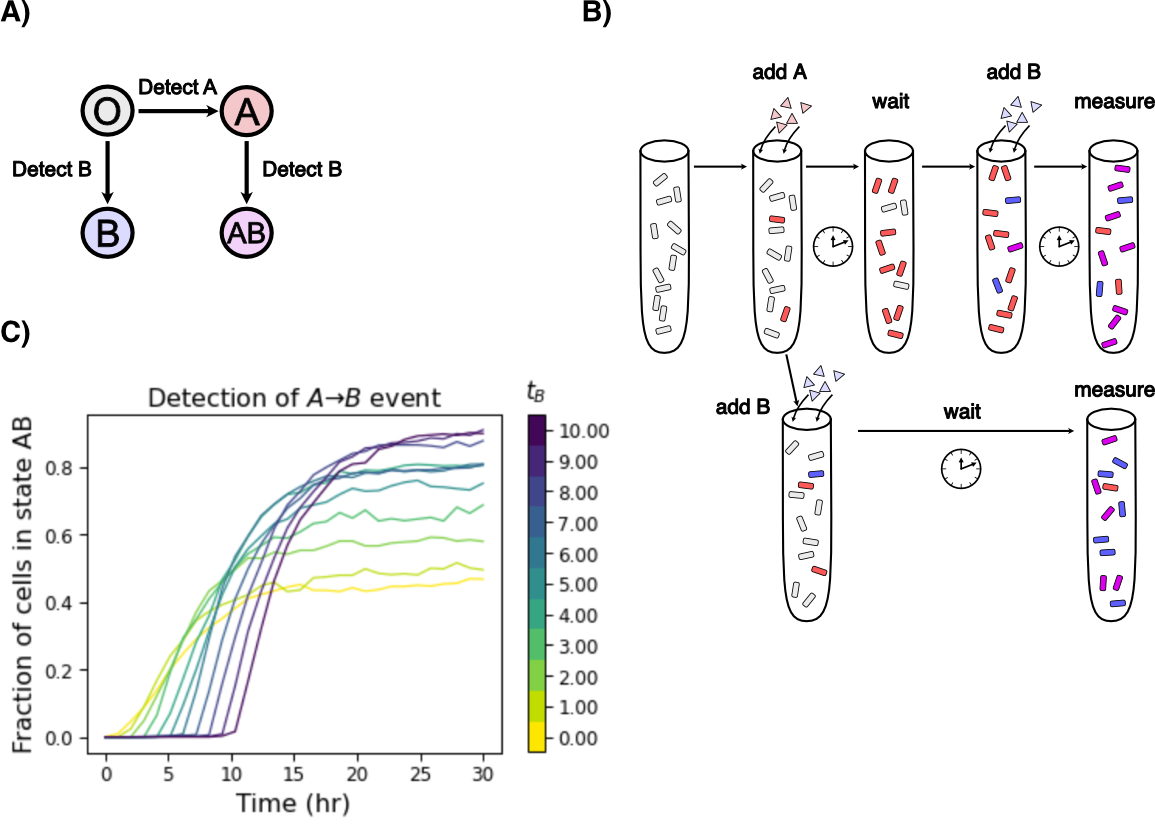
\includegraphics[scale=1]{figures/TLG_overview.png}
\caption{Overview of the temporal logic gate. \textbf{A)} State machine describing a single temporal logic gate unit. ``Detection'' is classically implemented with integrases whose activities are induced by signals $A$ and $B$. \textbf{B)} The behavior of a population of cells where each cell contains a single temporal logic gate. The final distribution of cell states can be used as a readout of the time delay between introduction of $A$ and introduction of $B$. \textbf{C)} Representative simulation of a genomically-integrated temporal logic gate (i.e., without explicitly replicating DNA species). Each curve is the fraction of cells in state $AB$ over time for a different delay time $t_B$ between introduction of $A$ and $B$.}
\label{fig:tlg_overview}
\end{figure}

A single cell expressing a temporal logic circuit is an imperfect sensor. Even if the cell is exposed to $A \Rightarrow B$, it is possible that it could, by stochastic fluctuation, not flip with integrase $intA$ for so long that it eventually runs into a $B$ molecule and integrates first with $intB$. The shorter the time delay between the introduction of $A$ and $B$, the more likely this sort of mis-firing will be. 

In a large population of temporal-logicl-circuit bearing cells, this imperfection can be exploited to create a population-level, analog measurement of not just which input appeared first, but the \emph{time delay} between the appearance of the two. If one input appears rapidly after the other, then many cells will ``misfire'' and report the wrong temporal value; if the two inputs are separated by a significant amount of time, then almost all cells will react to the first input before the second input arrives, and the population will homogeneously report the correct value. With proper calibration, the final distribution of cell states can be used to back out the time difference between inputs. 

Equivalently, this type of population-level circuit can be used to measure differences in \emph{concentration} of inputs that appear at the same time. 

Importantly, the population-level circuit assumes that each cell has a single, simple state. This is achieved by using a chromosomally-integrated reporter module, so that the cell has a single, unique state (or, at least, will after a round or two of division). One could easily imagine performing the same type of population-level measurement in a single cell by using a state-bearing plasmid with a high copy number. This could make the circuit much more compact, and potentially simpler to sample depending on the circuit's intended environment. 

Will a single-cell, plasmid-based temporal logic gate still perform as advertised? There are practical, integrase-related difficulties with making such a circuit -- as originally designed, multiple copies of the gate's reporter module would recombine in unexpected and unwanted ways -- but even setting those aside, moving a population-level circuit into a single cell adds new complications and sources of noise. For one thing, recording events between modules are no longer independent -- transcription of a single integrase mRNA can produce a number of module-flipping events. The frequency of a plasmid state in a cell might also not be stable over generations, due to random partitioning at division. 

A straightforward way to ask whether or not a single-cell temporal logic gate can still give analog measurements is to simulate it. To do so, we should use stochastic simulation (since stochastic fluctuations are likely important for plasmid dynamics) and we will need to model plasmid replication (since stateful plasmids are the principle species acted on by the circuit). 
	
\subsubsection{Is there \emph{really} no other way to model this circuit?}

You could probably get away with representing each cell as a finite Markov chain with transition rates fixed by the presence or absence of each signal molecule, with the state of the chain encoding the number of plasmids in that cell with each reporter state. This could be a good approximation \textit{if} you are sure you can approximate each cell's (and each plasmid's) internal dynamics with Markovian state transitions. You could easily add partitioning dynamics to this sort of model by splitting each cell at fixed intervals, with plasmids duplicated and binomially partitioned at division time.

What you will lose with the simpler Markov chain description of the temporal logic gate is the ability to couple the gate's activity to arbitrary dynamic gene networks. The example shown here arguably doesn't strictly need the full power of BioSCRAPE's stochastic molecular simulator, but it would not be difficult to imagine tying integrase activity to, for example, a feed-forward pulse generator, so that the gate only detects the $A\to B$ transition if $B$ appears within a short window after the appearance of $A$. 

\subsubsection{Does the temporal logic gate work when modeled on a replicating plasmid?}

It does, although with more noise than the original genome-located temporal logic gate. See Figure \ref{fig:tlg_results}. 

\begin{figure}[!ht]
\centering
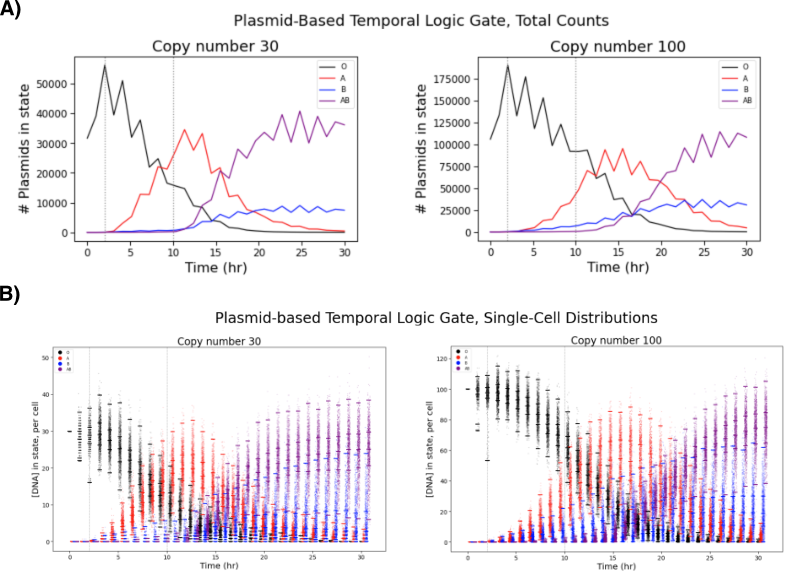
\includegraphics[scale=2]{figures/TLG_results.png}
\caption{The temporal logic gate on a replicating plasmid. \textbf{A)} Total counts of plasmids of copy number 30 or 100 in each state across a population of 1,056 cells introduced to $A$ at time 2 hours and $B$ at time 10 hours. \textbf{B)} Same data as in \textbf{A}, disaggregated into individual cells' copy numbers of plasmids in each state. Points are shifted and jittered slightly on the time axis for visibility. Solid ticks mark the 1st, 25th, 50th, 75th, and 99th percentile copy numbers for each state at each time.}
\label{fig:tlg_results}
\end{figure}

% DATA AVAILABILITY AND REPRODUCIBILITY
\section{Data/Code Availability and Reproducibility}

\subsection{What software did you use to simulate this stuff?}

All simulations were performed in Python using the BioSCRAPE cell simulator, with software and package versions given in Table \ref{tab:versions}. Copy number data from \cite{Shao2021} was extracted from Figure 1e using \href{https://automeris.io/WebPlotDigitizer/}{WebPlotDigitizer}).

\begin{table}[hbt!]
\centering
\begin{tabular}{lll}
\hline
Software/Package & Version\\
\hline
Python & 3.8.1\\
ipykernel & 5.1.4\\
IPython & 7.12.0\\
Jupyter Lab & 2.1.5\\
Numpy & 1.20.2\\
Matplotlib & 3.4.1\\
Scipy & 1.6.2\\
BioSCRAPE & 1.0.3\\
Noisyopt & 0.2.2\\
\hline
\end{tabular}
\caption{Software versions used for this report.}\label{tab:versions}
\index{tables}
\end{table}

For this document, code was run using a mid-2014 MacBook Pro running macOS 10.14.6. 

\subsection{Do you have code for any of this? Where can I get it?}

All code used in this document, along with examples and some additional analysis, can be found in the ``code'' folder in this document's GitHub repository at \url{https://github.com/sclamons/plasmid_replication_modeling}. All code is packaged as interactive Jupyter notebooks:

\begin{itemize}
	\item \textbf{summary\_table\_plots.ipynb}: Descriptions of the models, simulations of just replicating DNA, and parameterization. Used for Figure \ref{fig:model_trajectories}, Table \ref{tab:speed}, and most of the main table. Start here.
	\item \textbf{simple\_bp\_model\_reduction.ipynb}: Semi-rigorous derivations for reductions of the three-species ColE1 replication model (see Section \ref{sec:simple_bp_reduction}), along with simulations to back up those derivations. Used for Figure \ref{fig:model_reduction_examples}.
	\item \textbf{CRISPRessilator.ipynb}: Worked examples of the five-node CRISPRlator (see Section \ref{ss:CRISPRi}) with no replication mechanism, trivial replication, dummy-triggered replication, and the full and three-species ColE1 replication mechanisms, as well as simulations using dummy-triggered replication at a variety of copy numbers. Used for Figures \ref{fig:crispr_overview}, \ref{fig:crispr_results}, and \ref{fig:crispr_results_2}, and for Table \ref{tab:speed}.
	\item \textbf{temporal\_logic\_gate.ipynb}: Worked examples of the temporal logic gate (see Section \ref{ss:temporal_gate} either as a single-copy genomic circuit or as a plasmid-based circuit on DNA with dummy-triggered replication. Used for Figures \ref{fig:tlg_overview} and \ref{fig:tlg_results}, and Table \ref{tab:speed}.
\end{itemize}

You will need to install the BioSCRAPE package to run the example notebooks (``pip install bioscrape''). BioSCRAPE is a performance-optimized, Cython-based Python package for efficient ODE and SSA simulation of biocircuits. See \url{https://github.com/biocircuits/bioscrape} and \href{https://doi.org/10.1101/121152}{``Fast and flexible simulation and parameter estimation for synthetic biology using bioscrape''} for more information.

% Figure example

%\begin{figure}[h]
%\centering
%\includegraphics[scale=1]{activators_vs_repressors.pdf}
%\caption{Changes in expression when the concentrations of two regulators (an activator and a repressor) are changed under different regulator concentration regimes. Both the repressor and the activator change expression 10-fold (top table). At low saturation of target promoter by the regulators, the activated promoter is more sensitive to changes in regulator concentration than the regulated promoter (middle table). Conversely, at high target saturation, the activated promoter is more robust to changes in regulator concentration (bottom table).}
%\label{actvsrep}
%\end{figure}


%% References with bibTeX database:
%\section{References}

%\bibliographystyle{model1-num-names}
\bibliographystyle{plain}
\bibliography{plasmid_replication.bib}
\end{document}
